%\newcommand{\csharp}[1]{\mintinline{csharp}{#1}}

\newcommand{\pex}{\textsc{Pex}}
\newcommand{\predator}{\textsc{Predator}}
\newcommand{\dotnet}{\textsc{.NET}}
\newcommand{\clang}{\textsc{C}}
\newcommand{\vsharp}{\textsc{V\#}}

\newcommand\addrset{loc}
\newcommand\termset{term}
\newcommand\guardset{guard}

\newcommand\eqby[1]{\mathrel{\stackrel{\mbox{\normalfont\tiny #1}}{=}}}
\newcommand\eqdef{\eqby{def}}

\newcommand\aite{ite}
\newcommand\ite[3]{\aite(#1,#2,#3)}
\newcommand\Ite[3]{\aite\big(#1,#2,#3\big)}
\newcommand\pair[2]{\langle#1, #2\rangle}
\newcommand\paiR[2]{\big\langle#1, #2\big\rangle}
\newcommand\mg[2]{#1=#2}
\newcommand\nmg[2]{#1\neq#2}
\newcommand\li[1]{LI(#1)}
\let\emptyheap\varepsilon
\newcommand\agrec{Rec}
\newcommand\agmerge{Merge}
\newcommand\agcompose{\bigcirc}
\newcommand\GRec[1]{\agrec\big(#1\big)}
\newcommand\GMerge[1]{\agmerge\big(#1\big)}
\newcommand\GCompose[2]{#1\agcompose#2}
\newcommand\agho{App}
\newcommand\gapp[1]{\agho(#1)}
\newcommand\GApp[1]{\agho\big(#1\big)}
\newcommand\aunion{\texttt{UNION}}
\newcommand\union[1]{\aunion\big(#1\big)}
\newcommand\Union[1]{\aunion\Big(#1\Big)}
\newcommand\aderef{readStore}
\newcommand\readTerm{readTerm}
\newcommand\writeTerm{writeTerm}
\newcommand\afind{find}
\newcommand\find[5]{\afind(#1,#2,#3,#4,#5)}
\newcommand\finD[5]{\afind\big(#1,#2,#3,#4,#5\big)}
\newcommand\Find[5]{\afind\Big(#1,#2,#3,#4,#5\Big)}
\newcommand\deref[2]{\aderef(#1,#2)}
\newcommand\Deref[2]{\aderef\big(#1,#2\big)}
\newcommand\compose[2]{#1\circ#2}
\newcommand\lmbd[2]{\lambda #1.#2}
\newcommand\lmbdx[1]{\lambda x.#1}
\newcommand\dom[1]{dom(#1)}
\newcommand\Dom[1]{dom\big(#1\big)}

\newcommand\Li[1]{LI\big(#1\big)}
\newcommand\amutate{writeStore}
\newcommand\amutateStack{writeStack}
\newcommand\mutate[3]{\amutate(#1,#2,#3)}
\newcommand\mutateStack[4]{\amutateStack(#1,#2,#3,#4)}
\newcommand\rdbodyext[6]{\Union{\big\{\paiR{#4\mg{#1}{#5}}{#6\big(#2(#5), xs\big)} \mid #5\in\dom{#2} \big\}\\&\qquad\qquad\qquad\cup\paiR{#4\bigwedge_{\mathclap{#5\in\dom{#2}}}{\nmg{#1}{#5}}}{#6\big(#3, xs\big)}}}
\newcommand\rdbody[4]{\rdbodyext{#1}{#2}{#3}{}{l}{#4}}
\newcommand\wrtbody[6]{\Union{&\paiR{\mg{#1}{#2}}{\writeTerm\big(#3,#4,#6\big)},
    \\&\paiR{\nmg{#1}{#2}}{\writeTerm\big(#5(#1),#4,#6\big)}}}
\newcommand{\var}[1]{\mathit{#1}}

\title{Неразрешиомсть задачи выполнимости ограничений номинальной системы типов с вариантностью}

\author{Мисонижник Александр Владимирович}

\authorrunning{Мисонижник Александр Владимирович}

\tocauthor{Мисонижник А.В.}
\institute{Санкт-Петербургский государственный университет\\
	\email{misonijnik@gmail.com}}

\lstset{style=sharpc, escapeinside={(*}{*)}}

\newfloat{Listing}{hbtp}{lop}
\newfloat{Figure}{hbtp}{lop}

\theoremstyle{plain}
%\newtheorem{thm}{Теорема}%[section]
%\newtheorem{lem}{Лемма}%[section]
\%newtheorem{crlr}{Следствие}%[section]

\theoremstyle{definition}
%\newtheorem{defn}{Определение}
%\newtheorem{remk}{Замечание}
%\newtheorem{prop}{Предложение}
%\newtheorem{exmp}{Пример}
\newtheorem*{proof*}{Доказательство}

\renewcommand{\defnautorefname}{Definition}
\renewcommand{\lemautorefname}{Lemma}
\renewcommand{\remkautorefname}{Remark}
\renewcommand{\propautorefname}{Proposition}
\renewcommand{\exmpautorefname}{Example}
\renewcommand{\thmautorefname}{Theorem}
\newcommand{\crlrautorefname}{Corollary}
\renewcommand{\sectionautorefname}{Section}
\newcommand{\Listingautorefname}{Listing}
\newcommand{\Figureautorefname}{Figure}

\maketitle


\begin{abstract}
Известно, что наибольшую сложность в области верификации программ представляет задача доказательства корректности программ с циклическими участками кода. Опираясь на подход символьного исполнения программ и на введенные формализмы обобщённых куч в работе~\cite{kostyukov2018csewu}, данная работа представляет алгоритм композиционального символьного исполнения без раскрутки отношения перехода программ с произвольным графом потока управления. На его основе был реализован символьный интерпретатор языка CIL в проекте V\#, символьной виртуальной машине для анализа .NET. Была проведена апробация алгоритма на примерах, включающих сложные потоки управления, и интерпретатора на тестовой базе проекта VSharp.Test и на библиотеке Chess.NET.
\end{abstract}

\section*{Введение}
Поиск путей в графе с ограничением в виде формальных языков~\cite{FLCpathProblem} --- это задача, в которой формальные языки используются для задания множества искомых путей. В таком подходе каждый путь соответствует слову, состоящему из меток его рёбер, а ограничением на путь является принадлежность соответствующего ему слова некоторому заданному формальному языку.

В качестве класса формальных языков по иерархии Хомского наибольший интерес представляют контекстно-свободные языки. В отличие от регулярных они обладают большей выразительностью. Поэтому в задаче поиска путей контекстно-свободные ограничения позволяют задавать более сложные отношения между вершинами. Так, например, важный класс запросов поиска вершин, лежащих на одном уровне иерархии~\cite{zhlang-2016}, задаётся только контекстно-свободными, но не регулярными ограничениями. Запросы такого вида, как и другие запросы с контекстно-свободными ограничениями имеют широкое применение в биоинформатике~\cite{bio-application} и при обработке rdf-файлов~\cite{zhlang-2016}.

Наиболее удобным и подходящим инструментом для работы с граф\-структурированными данными являются графовые базы данных. Так же как и реляционные, графовые базы данных поддерживают свой язык запросов. С его помощью графовые базы данных позволяют решать вышеупомянутую задачу поиска путей. Но ограничения на пути, которые поддерживается в наиболее распространённых базах данных, являются в лучшем случае регулярными.

Отсутствие поддержки контекстно-свободных ограничений в графовых базах данных, во-первых, сильно ограничивает выразительность языка запросов. Во-вторых, при необходимости в более сложных запросах разработчикам приходится самим писать алгоритмы, решающие задачу контекстно-свободной достижимости для их частного случая. Так, например, Хуэй Мяо и др.~\cite{datascince-lifecycle} разработали систему хранения и отслеживания версий артефактов, возникающих при научных работах. Вся информация про артефакты хранилась в графовой базе данных. При этом при разработке возникла потребность в выполнении запросов с контекстно-свободными ограничениями для выявления взаимоотношений между различными версиями различных артефактов. Это и послужило началом статьи~\cite{datascince-lifecycle}, в которой приводятся алгоритмы решения частных запросов.

В недавнем исследовании Йохем Куйперс и др.~\cite{Kuijpers:2019:ESC:3335783.3335791} произвели сравнительный анализ наиболее известных алгоритмов поиска путей с конте\-кстно-свободными ограничениями. Алгоритмы запускались на графах, находящихся в хранилище графовой базы данных Neo4j. По результатам исследования было показано, что в контексте Neo4j алгоритмы обладают большим временем работы, и поэтому дальнейшая работа по расширению языка запросов прекратилась. При этом Рустам Азимов~\cite{Azimov:2018:CPQ:3210259.3210264} предоставил матричный алгоритм и его реализацию, которая работает за разумное время на реальных данных. Но, так как алгоритм был реализован вне контекста базы данных, его результат приняли недостаточно показательным. Поэтому вопрос о реализуемости запросов с контекстно-свободными ограничениями в графовых базах данных, а соответственно и о возможности расширения языка запросов для их поддержки остаётся открытым.

\section{Постановка задачи}
Целью данной работы является полная поддержка запросов с конте\-кстно-свободными ограничениями для графовой базы данных. А именно, необходимо предоставить пользователю возможность формулировать запросы с контекстно-свободными ограничениями в терминах одного из существующих стандартных языков запросов и исполнять их в графовой базе данных за приемлемое время. Для достижения этой цели были поставлены следующие задачи.

\begin{itemize}
    \item Выполнить обзор существующих реализаций поддержки запросов с контекстно-свободными ограничениями в графовых базах данных. В результате обзора необходимо выбрать наиболее перспективный с точки зрения производительности алгоритм решения задачи контекстно-свободной достижимости и подходящую для его интеграции базу данных. При выборе базы данных необходимо учитывать как возможность интеграции выбранного алгоритма, так и возможность поддержки одного из стандартных языков запросов, позволяющего выражать контекстно-свободные ограничения.
    \item Интегрировать выбранный на предыдущем шаге алгоритм в выбранную графовую базу данных.
    \item Расширить язык запросов выбранной базы данных конструкциями, необходимыми для выражения контекстно-свободных ограничений.
    \item Произвести замеры производительности полученного решения и сравнить его с существующими решениями.
\end{itemize}


\section{Обзор}

\subsection{Терминология}
Контекстно-свободной грамматикой называется $G = (\Sigma, N, P, S)$, где $\Sigma$ --- алфавит терминальных символов, $N$ --- алфавит нетерминальных символов, $P$ --- множество правил вида $A \rightarrow \alpha$, где $A \in N$, $\alpha \in (\Sigma \cup N)^*$, а $S \in N$ --- выделенный стартовый нетерминал.

% \gsv{про S забыли}.

Языком $L$ над алфавитом $\Sigma$ называется любое подмножество $2^{\Sigma^*}$. Языком, порождаемой грамматикой G, является множество $L(G) = \{S \xRightarrow{*} \beta, \beta \in \Sigma^*\}$, где $S \xRightarrow{*} \beta$ означает, что из нетереминала $S$ путём последовательного применения правил грамматики выводится $\beta$.

Контекстно-свободная грамматика $G = (\Sigma, N, P, S)$ находится в осла\-бленной нормальной форме Хомского, если любое её правило имеет вид $A \rightarrow BC$, где $A, B, C \in N$, либо $A \rightarrow a$, где $A \in N, a \in \Sigma$. В отличие от нормальной формы Хомского в ослабленной, во-первых, допускается присутствие стартового нетерминала $S$ в правых частях правил грамматики, во-вторых, запрещаются правила вида $S \rightarrow \epsilon$, где $\epsilon$ --- пустая строка.

% \gsv{Это не нормальная форма Хомского. У НФХ есть дополнительные ограничения. Мы называем то, что здесь, ослабленной НФХ. Важно отдельно проговорить разницу с НФХ.}

В задаче поиска путей с ограничениями в виде формальных языков дан граф $(V, E)$, разметка его рёбер $l: E \rightarrow \Sigma$ и язык $L$ над алфавитом $\Sigma$. Требуется найти множество всех пар вершин, между которыми существует путь, метки на рёбрах которого образуют слово в заданном языке. То есть требуется найти следующее множество:
\[\{(v, to): \exists p=(e_1,...,e_n) \in E^*: l(e_1)...l(e_n) \in L,~src(e_1)=v,~dst(e_n)=to\}\]
Здесь $src(e)$ и $dst(e)$ для $e \in E$ означают начальную и конечную вершину ребра $e$. В данном контексте язык $L$ называется языком ограничений.
% \gsv{У Вас вершины v и to никак с путём не связаны}

Задача поиска путей с контекстно-свободными ограничениями --- это задача поиска путей в виде формальных языков, в которой язык задаётся контекстно-свободной грамматикой.

\subsection{Графовые базы данных}
Графовые СУБД\footnote{СУБД --- Система управления базами данных} (далее просто графовые базы данных) --- это разновидность СУБД, в которой данные хранятся в виде графов. В отличие от других разновидностей, в графовых базах данных отношения между объектами так же важны, как и сами объекты.

Основной моделью представления графов в таких базах данных является gpraph property model~\cite{graph-propery-model}. В ней каждая сущность может содержать набор свойств в формате ключ-значение. Основными сущностями являются узлы и отношения. Узлы соответствуют вершинам графа и помимо свойств могут иметь несколько меток. Отношения соответствуют рёбрам и имеют ровно одну метку, которая называется типом отношения. На рисунке~\ref{fig:graph_bd_1} показан небольшой пример графа в такой модели. 

\begin{figure}[h]
\centering
    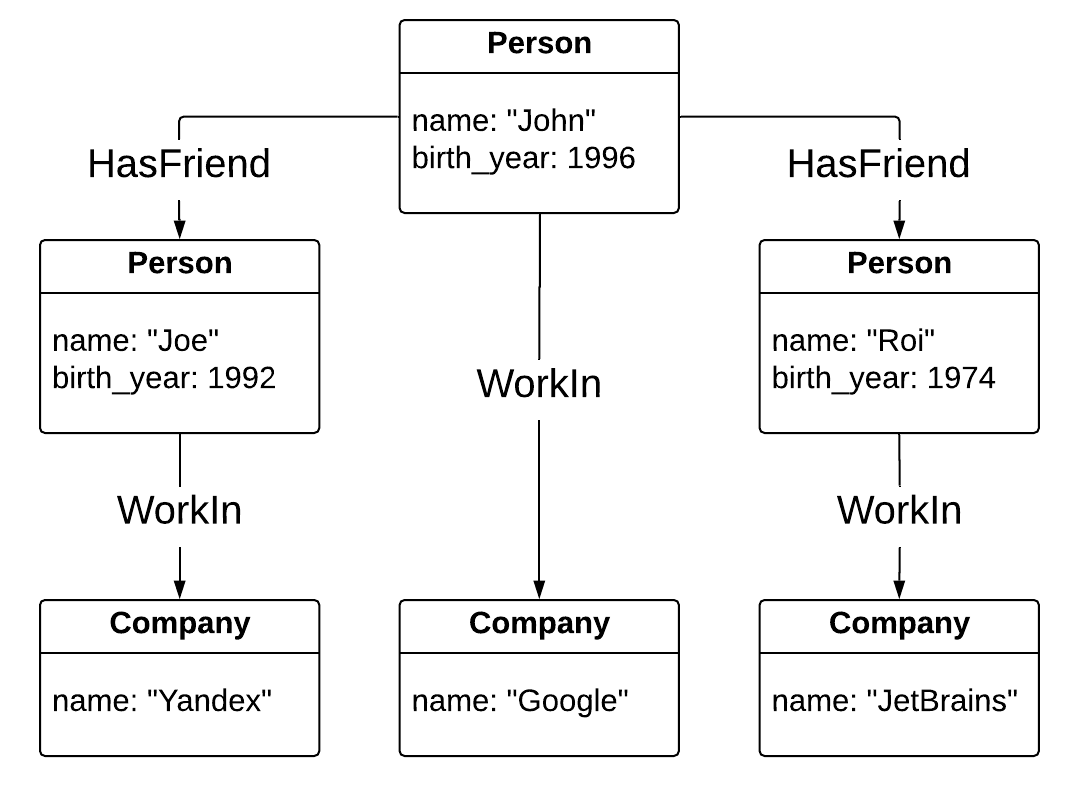
\includegraphics[width=0.7\linewidth]{Terekhov/pictures/graph_bd_1.png}
    \caption{Пример социального графа}
    \label{fig:graph_bd_1}
\end{figure}

Для работы с графами графовые базы данных предоставляют язык запросов, самым популярным из которых является Cypher~\cite{cypher-language}. В нём главный интерес представляют запросы вида сопоставления с образцом. Они позволяют задавать интересующие пути или подграфы в виде шаблонов и описывать информацию, которую нужно извлечь после удачного сопоставления. На рисунке~\ref{code:cypher_query} приведён пример такого запроса. Шаблон пути описывается в выражении MATCH. В нём между круглыми скобками задаются шаблоны вершин, а между квадратными шаблоны рёбер. Таким образом в данном примере задаются следующие ограничения: путь должен начинаться из вершины с меткой Person и именем John и состоять из двух рёбер, первое из которых должно иметь тип HasFriend, а второе WorkIn. В выражении RETURN задаётся информация, которую нужно извлечь. В данном примере это имя последней в пути вершины. В итоге ответом на такой запрос являются имена компаний, в которых работают друзья Джона. Результатом работы этого запроса на графе из рисунка~\ref{fig:graph_bd_1} является множество \{"Yandex", "JetBrains"\}.

%\lstset{
%   basicstyle=\fontsize{14}{14}\selectfont\ttfamily
%}

\begin{figure}[h]
\begin{lstlisting}[language=sql]
MATCH (p:Person)-[:HasFriend]->()-[:WorkIn]->(to)
WHERE p.name = "John"
RETURN to.name
\end{lstlisting}
\caption{Пример конечного запроса на языке Cypher}
\label{code:cypher_query}
\end{figure}

С формальной точки зрения шаблоны пути в выражении MATCH позволяют поставить задачу поиска путей с ограничениями в виде формальных языков. Так в запросе на рисунке~\ref{code:cypher_query} языком ограничений является конечный язык $\{(HasFriend, WorkIn)\}$. Для запроса на рисунке~\ref{code:cypher_query_2} ограничением является регулярный язык $\{A, B\}^*$. 

\begin{figure}[h]
\begin{lstlisting}[language=sql]
MATCH (v)-[:A | :B *]->(to)
RETURN to.name
\end{lstlisting}
\caption{Пример регулярного запроса на языке Cypher}
\label{code:cypher_query_2}
\end{figure}

При этом регулярные ограничения поддерживаются лишь частично и позволяют искать только пути произвольной длины с заданными метками на рёбрах, а более глубокие регулярные выражения не поддерживаются. Поэтому на текущий момент язык запросов довольно ограничен.

\subsection{Существующие решения}
Как было упомянуто раннее, ни одна графовая база данных не поддерживает запросов с контекстно-свободными ограничениями. Тем не менее существуют альтернативные решения поддержки таких запросов. 

\subsubsection{Парсер-комбинаторы для Neo4j}\label{sec:pareser-combinators}
В 2018 году группой исследователей из JetBrains Research на основе библиотеки Meerkat была разработана библиотека для поддержки запросов с контекстно-свободными ограничениями~\cite{parser-combinators}. Она использует графовую базу данных Neo4j~\cite{neo4j} как хранилище графов и позволяет задавать запросы в виде парсер-комбинаторов. Основным достоинством данной работы является то, что с помощью этой библиотеки кроме контекстно-свободных запросов можно выразить базовую часть языка Cypher. Но так как конкурировать с оригинальной реализацией выполнения запросов Neo4j очень сложно, это достигается вместе c сильной потерей производительности. Кроме этого контекстно-свободные запросы обрабатываются также достаточно медленно.

Таким образом данное решение является альтернативой языка запросов Neo4j, а не его расширением. Из-за медленного времени работы такое решение подходит только для работы с небольшими графами. 

\subsubsection{Расширение языка запросов SPARQL}\label{subsection:cypher-extention-2}
%Про sparql%
В 2016 Сяованг Чжан предоставил язык cfSPARQL~\cite{zhlang-2016} --- расширение языка SPARQL, который способен выразить запросы с контекстно-свободными ограничениями. Также он привёл алгоритм для вычисления таких запросов и замеры производительности. Но, во-первых, работа была сделана вне контекста графовой базы данных, а во-вторых, время работы предложенного алгоритма было больше, чем время работы парсер-комбинаторов.

\subsubsection{Существующие реализации алгоритмов решения задачи контекстно-свободной достижимости}
Основной сложностью расширения языка запросов для поддержки запросов с контекстно-свободными ограничениями является долгое время работы соответствующих алгоритмов. Так, например, в 2019 году Йохем Куйперс и другие исследователи с целью попытки расширения языка запросов Cypher для графовой базы данных Neo4j произвели сравнительный анализ производительности наиболее известных алгоритмов решения задачи контекстно-свободной достижимости.

В данном исследовании были рассмотрены и произведены замеры времени работы алгоритма Элле Хелингса~\cite{hellings-2015}, основанного на атрибутных грамматиках, восходящего алгоритма Фреда Сантоса~\cite{santos-2018}, матричного алгоритма Рустама Азимова~\cite{Azimov:2018:CPQ:3210259.3210264} и алгоритма Петтери Севона~\cite{bio-application}. Все алгоритмы были интегрированы в Neo4j и запускались на графах, находящихся в её хранилище. Алгоритмы были написаны на языке Java, при этом их реализация являлась однопоточной.

% \gsv{В таких местах надо сразу ссылку на алгоритм давать.}

По результатам замеров производительности было показано, что время работы алгоритмов является слишком большим и неприемлемым для широкого практического использования. Поэтому дальнейшая работа по интеграции и расширению языка запросов была приостановлена.

Тем не менее, матричный алгоритм Рустама Азимова в сравнительном анализе Йохема Куйперса был реализован без необходимых матричных библиотек, которые могут сильно уменьшить время его работы. Так, например, в исследовании Никиты Мишина и др.~\cite{azimov-evalution} был произведён сравнительный анализ времени работы нескольких реализаций алгоритма Рустама Азимова, основанных на различных специализированных матричных библиотеках. Графы и запросы к ним были взяты из объемлющего набора данных CFPQ\_Data~\cite{cfpq-data}, предоставленного лабораторией языковых инструментов JetBrains Research. 

Результаты замеров Никиты Мишина и др. показали, что при грамотной реализации алгоритма Рустама Азимова и использовании подходящих матричных библиотек можно добиться очень высокой производительности. Поэтому, так как основной проблемой применимости запросов с контекстно-свободными ограничениями является долгое время работы соответствующих алгоритмов, в качестве алгоритма решения задачи конте\-кстно-свободной достижимости был выбран матричный алгоритм Рустама Азимова.

\subsection{Матричный алгоритм Рустама Азимова}\label{sec:matrix-algo}
Выбранный в предыдущей главе алгоритм Рустама Азимова~\cite{Azimov:2018:CPQ:3210259.3210264}, в отличие от других алгоритмов решения задачи контекстно-свободной достижимости~\cite{hellings-2015, santos-2018, zhlang-2016}, работает с графами в виде разреженных матриц смежности. Данный алгоритм состоит из последовательности операций над разреженными матрицами, время работы которых зависит не от размеров матричных операндов, а от количества их ненулевых элементов.

На вход алгоритму (см. алгоритм 1) поступает помеченный граф $D=(V,E)$ и контекстно-свободная грамматика $G=(\Sigma, N, P, S)$ в ослабленной нормальной форме Хомского. Для каждого нетерминала $A$ в ассоциативном массиве $T$ хранится соответствующая ему булева матрица $T[A]$. На всём этапе алгоритма поддерживается следующий инвариант: $T[A]_{i,j} = 1$ равносильно существует пути, метки на рёбрах которого образуют слово, выводящееся из нетерминала $A$. На первом этапе происходит инициализация матриц с помощью простых правил грамматики, после чего инвариант выполняется для всех путей единичной длины. На втором этапе происходит транзитивное замыкание, после чего этот инвариант верен для всех путей. Результатом данного алгоритма является матрица, соответствующая стартовому нетерминалу $S$.

%  Это позволяет для его реализации использовать многопоточные матричные библиотеки, с помощью которых можно добиться очень высокой производительности. Поэтому на текущий момент алгоритм Рустама Азимова показывает наилучшее время работы на практике.

\begin{algorithm}
\caption{Матричный алгоритм Рустама Азимова}

\begin{algorithmic}[1]
\Function{contextFreePathQuerying}{$D$, $G$}
    \State{$n =$ getNodeCount(D)}
    \State{$N =$ getAllNonterms(G)}
    \State{$E =$ getEdges($D$)}
    \State{$P =$ getRules($G$)}
    \State{$S =$ getStartNonterm($G$)}
    \State{$T = \{A \rightarrow \varnothing_{n \times n} : A \in$ $N$ \} }
    \ForAll{$(v, to, label) \in E$}
    \Comment{Инициализация матриц}
        \ForAll{$A \rightarrow label \in P$}
            \State{$T[A]_{i,j} = 1$}
        \EndFor
    \EndFor    
    \While{$\exists A: T[A]$ is changing}
    \Comment{Вычисление замыкания}
        \ForAll{$A \rightarrow BC \in P$}
            \State{$T[A] \oplus= T[B] \otimes T[C]$}
        \EndFor
    \EndWhile
\State \Return $T[S]$
\EndFunction

\end{algorithmic}
\end{algorithm}

Практическое время работы алгоритма Рустама Азимова сильно зависит от производительности используемой матричной библиотеки. Это накладывает некоторые ограничения на выбор подходящей графовой базы данных, так же как и возможность представления графов в матричном виде.

\subsection{RedisGraph}
RedisGraph~\cite{redis-graph} --- это высокопроизводительная графовая база данных, поддерживающая язык запросов Cypher. В отличие от наиболее распространённой графовой базы данных Neo4j~\cite{neo4j}, RedisGraph написан на языке Си и для работы с данными использует Redis~\cite{redis}, основным достоинством которого является возможность хранить данные прямо в оперативной памяти. Это позволяет RedisGraph быстро обрабатывать пользовательские запросы.

Также RedisGraph является единственной графовой базой данных, которая работает с графами в виде разреженных матриц смежности и транслирует запросы языка Cypher в матричные выражения. Для представления графов в таком виде и работы с ними в терминах линейной алгебры используется мощный матричный фреймворк GraphBlas~\cite{graph-blas}. Его реализация SuiteSparse~\cite{suite-sparse} является многопоточной и сильно оптимизирована, что позволяет RedisGraph добиться высокой производительности.

Из всего этого следует, что RedisGraph идеально подходит для интеграции матричного алгоритма. Во-первых, графы представляются в необходимом алгоритму виде, что позволит избежать издержек на конвертацию форматов. Во-вторых, использование SuiteSparse для вычисления матричных операций позволит добиться высокой производительности. Поэтому RedisGraph был выбран в качестве графовой базы данных для интеграции матричного алгоритма и расширения языка запросов.

% Так как алгоритм Рустама Азимова работает с матричным представлением графа,, как наиболее подходящий для интеграции матричного алгоритма.

\subsection{Расширение языка Cypher}\label{subsection:cypher-extention}
На текущий момент оригинальная версия языка Cypher, используемая в том числе и в RedisGraph, не поддерживает запросов с контекстно-свободными ограничениями. Но тем не менее в 2017 году был разработан черновой вариант спецификации расширения Cypher~\cite{cypher-specification}, которая вводит в язык шаблоны путей. Они позволяют выразить более сложные запросы, в том числе запросы с контекстно-свободными ограничениями.

Шаблоны путей являются альтернативой шаблонам рёбер, которые есть в оригинальном Cypher. Они, как и шаблоны рёбер, могут встречаться в выражении MATCH и иметь своё направление. Кроме этого в глобальной области запроса им можно задавать имя, на которое потом можно ссылаться внутри других шаблонов.

Шаблон пути представляет из себя регулярное выражение над некоторыми примитивами. В качестве таких примитивов могут выступать шаблоны рёбер, шаблоны вершин и ссылки на именованные шаблоны путей. Также любым подвыражениям можно задавать своё направление. Основная часть конкретного синтаксиса данного расширения приведена на рисунке~\ref{fig:cypher_syntax}.

\begin{figure}[]
\begin{align*}
\begin{split}
PathPattern     &= ["<"],~"-/",~PathExpression,~"/-",~[">"]\\
PathExpression  &= \{PathAlternative\}\\
PathAlternative &= PathRepetition,~\{"|", PathRepetition\}\\
PathRepetition  &= ["<"],~PathBase,~[">"],~("*")
\end{split}\\
\begin{split}
PathBase &= PathEdge \\
         &~~|~PathNode \\
         &~~|~PathReference \\
         &~~|~"[",~PathExpression,~"]"
\end{split}\\
\begin{split}
PathEdge      &= Label \\
PathNode      &= "(",~[Label,~\{"|",~Label\}],~")" \\
PathReference &= "\sim",~SymbolicName; \\
Label         &= ":",~LabelName
\end{split}
\end{align*}
\caption{Расширение конкретного синтаксиса Cypher}
\label{fig:cypher_syntax}
\end{figure}

Каждый шаблон пути задаёт отношение на множестве вершин. Поэтому семантикой языка шаблонов путей $L_{P}$ в контексте графа $G(V, E)$ является отображение $\llbracket \cdot \rrbracket_{G}: L_P \rightarrow V \times V$, которое каждому шаблону $p\in L_P$ сопоставляет множество пар вершин, между которыми существует путь, удовлетворяющий данному шаблону $p$. 

Подробное описание данной семантики приводится в таблице~\ref{tab:cypher_sematic}.  В ней наибольший интерес представляют именованные шаблоны путей, так как именно с помощью них можно выразить запросы с контекстно-свободными ограничениями. Все именованные шаблоны путей $S_i = p_j$ можно рассматривать как правила контекстно свободной грамматики с алфавитом нетерминалов $\{S_i\}_{i=1}^n$. Тогда каждый нетерминал $S_j$ порождает язык $L_{S_j} \subset L_p$, а семантикой соответствующего именованного шаблона пути $S_j=p_j$ является множество $\bigcup\limits_{p \in L_{s_j}} \llbracket p \rrbracket_{G}$.

На рисунке~\ref{code:cypher_query_3} приведён пример запроса в расширенном синтаксисе. В нём декларируется именованный шаблон S, который задаёт множество правильных скобочных последовательностей над ребрами с типом L и R. Далее в выражении MATCH задаётся шаблон пути, состоящий из ссылки на шаблон S. Таким образом результатом обработки запроса является множество всех пар вершин, между которыми существует путь, метки на рёбрах которого образуют правильную скобочную последовательность. 

\begin{table}[h!]
\begin{adjustbox}{max width=\textwidth}
\begin{tabular}{|c|c|c|}
\hline
$p \in L_P$                                                                                  & $\llbracket p \rrbracket_{G}$                                                                                                                                                                                   & Описание шаблона пути                                                                                                         \\ \hline
\hline
()                                                                                            & $\{(v, v): v \in V\}$                                                                                                                                                                                           & \begin{tabular}[c]{@{}c@{}}Пустой путь, состоящий из \\ одной произвольной вершины\end{tabular}                               \\ \hline
:a                                                                                            & $\{e=(v,to): e \in E, type(e)=a\}$                                                                                                                                                                              & \begin{tabular}[c]{@{}c@{}}Путь единичной длины,\\  состоящий из ребра с типом $a$\end{tabular}                               \\ \hline
(:b)                                                                                          & $\{(v, v): v \in V, label(v)=b\}$                                                                                                                                                                               & \begin{tabular}[c]{@{}c@{}}Пустой путь, состоящий из одной\\  вершины, помеченной меткой $b$\end{tabular}                     \\ \hline
$\alpha~\beta$                                                                                & $\llbracket \alpha \rrbracket_{G}\circ \llbracket \beta \rrbracket_{G}$                                                                                                                                         & Конкатенация путей $\alpha$ и $\beta$                                                                                         \\ \hline
$\alpha~|~\beta$                                                                              & $\llbracket \alpha \rrbracket_{G}\cup \llbracket \beta \rrbracket_{G}$                                                                                                                                          & Альтренатива между путями $\alpha$ и $\beta$                                                                                  \\ \hline
$[\alpha]$                                                                                    & $\llbracket \alpha \rrbracket_{G}$                                                                                                                                                                              & \begin{tabular}[c]{@{}c@{}}Квадратные скобки позволяют \\ группировать  выражения \\ для задания ассоциативности\end{tabular} \\ \hline
\textless{}$\alpha$                                                                           & $\{(to, v): (v, to) \in \llbracket \alpha \rrbracket_{G}\}$                                                                                                                                                     & Путь, обратный к пути $\alpha$                                                                                                \\ \hline
\textless{}$\alpha$\textgreater{}                                                             & $\llbracket \alpha~|~$\textless{}$\alpha \rrbracket_{G} $                                                                                                                                                       & \begin{tabular}[c]{@{}c@{}}Альтернатива между путём $\alpha$ и\\ обратным к нему\end{tabular}                                 \\ \hline
$\alpha^*$                                                                                    & $\llbracket \alpha \rrbracket_{G}^{*}$                                                                                                                                                                          & \begin{tabular}[c]{@{}c@{}}Путь, состоящий из\\ конкатенации 0 или более путей $\alpha$\end{tabular}                          \\ \hline
\begin{tabular}[c]{@{}c@{}}$\{S_i = p_i\}_{i=1}^{n}$\\ -- named\\  path patterns\end{tabular} & \begin{tabular}[c]{@{}c@{}}$P = \{S_i \rightarrow p_i\}_{i=1}^n$\\ $Gram_j = (\Sigma, \{S_i\}_{i=1}^n, P, S_j)$\\ $\llbracket S_j \rrbracket_{G} = \bigcup\limits_{p \in L(G)}{\llbracket p \rrbracket_{G}}$\end{tabular} & Именнованые шалоны путей                                                                                                      \\ \hline
$\sim$$S$                                                                                     & $\llbracket S \rrbracket_{G}$                                                                                                                                                                                   & \begin{tabular}[c]{@{}c@{}}Ссылка на именнованный\\  шаблон пути\end{tabular}                                                 \\ \hline
\end{tabular}
\end{adjustbox}
\caption{Семантика языка шаблонов путей}
\label{tab:cypher_sematic}
\end{table}

\begin{figure}[h!]
\begin{lstlisting}[language=sql]
PATH PATTERN S = ()-/ [:L ~S :R] | [~S ~S] | () /-()
MATCH (v)-/ ~S /-(to)
RETURN v, to
\end{lstlisting}
\caption{Пример запроса в расширенном синтаксисе Cypher}
\label{code:cypher_query_3}
\end{figure}

Данная спецификация расширения Cypher была представлена официальными разработчиками и сильно расширяет выразительность языка, предоставляя удобную возможность выражать запросы как с регулярными, так и с контекстно-свободными ограничениями. Поэтому в моей работе приводится поддержка выполнения запросов именно для этого расширения языка.

% \gsv{Не хватает какого-то чёткого вывода про то, что вот именно это мы и буем использовать.}

\section{Реализация}
По результатам обзора было решено реализовать поддержку расширения языка Cypher, представленную в главе~\ref{subsection:cypher-extention}, для графовой базы данных RedisGraph. За основу алгоритма, решающего задачу поиска путей с контекстно-свободными ограничениями, был взят матричный алгоритм Рустама Азимова, описанный в главе~\ref{sec:matrix-algo}.

% \gsv{И зжесь надо ещё раз подитожить в духе "по результатм обзора было решено сделать то и это с использованием того и сего"}

\subsection{План выполнения запроса}\label{execution-plan}
В RedisGraph основной частью обработки запроса является построение плана его выполнения. Её часть, которая относится к шаблонам путей приведена на рисунке~\ref{fig:execution_plan}. В ней зелёным цветом выделено то, что было добавлено или расширено.

В самом начале, после получения запроса строится его абстрактное синтаксическое дерево \textit{AST}. Далее, из него извлекаются именованные и неименованные шаблоны путей \textit{PathPattern} и \textit{NamedPathPatterns}, после чего они преобразуются в более удобное промежуточное представление \textit{PathExpr}. При этом, для дальнейшего связывания ссылок, именованные шаблоны сохраняются в глобальном контексте запроса \textit{PathPatternCtx}.

На следующем этапе происходит трансляция промежуточных представлений \textit{PathExpr} в матричные выражения \textit{AlgebraicExpression}. В них операндами являются либо матрицы, полученные из указанного в запросе графа \textit{GraphCtx}, либо ссылки на именованные шаблоны путей из \textit{PathPatternCtx}. Основной идеей трансляции является то, что после вычисления матричного выражения получается матрица, которая задаёт то же самое отношение на множестве вершин, что и исходный шаблон пути.

Далее каждое такое выражение формирует новую операцию плана выполнения запроса \textit{CfpqTraverseOp}. При её вычислении сначала происходит запуск расширенной версии матричного алгоритма Рустама Азимова. Он решает задачу контекстно-свободной достижимости, заданной именованными шаблонами путей. После этого все ссылки в матричном выражении заменяются на полученные в ходе алгоритма матрицы и происходит вычисление матричного выражения. Каждая такая операция добавляется в план выполнения запроса.

%  \gsv{Используйте \textit{CfpqTraverseOp} вместо долларов для длинных слов. Они тогда не распадаются из-а лишних пробелов.}

\begin{figure}[H]
\centering
    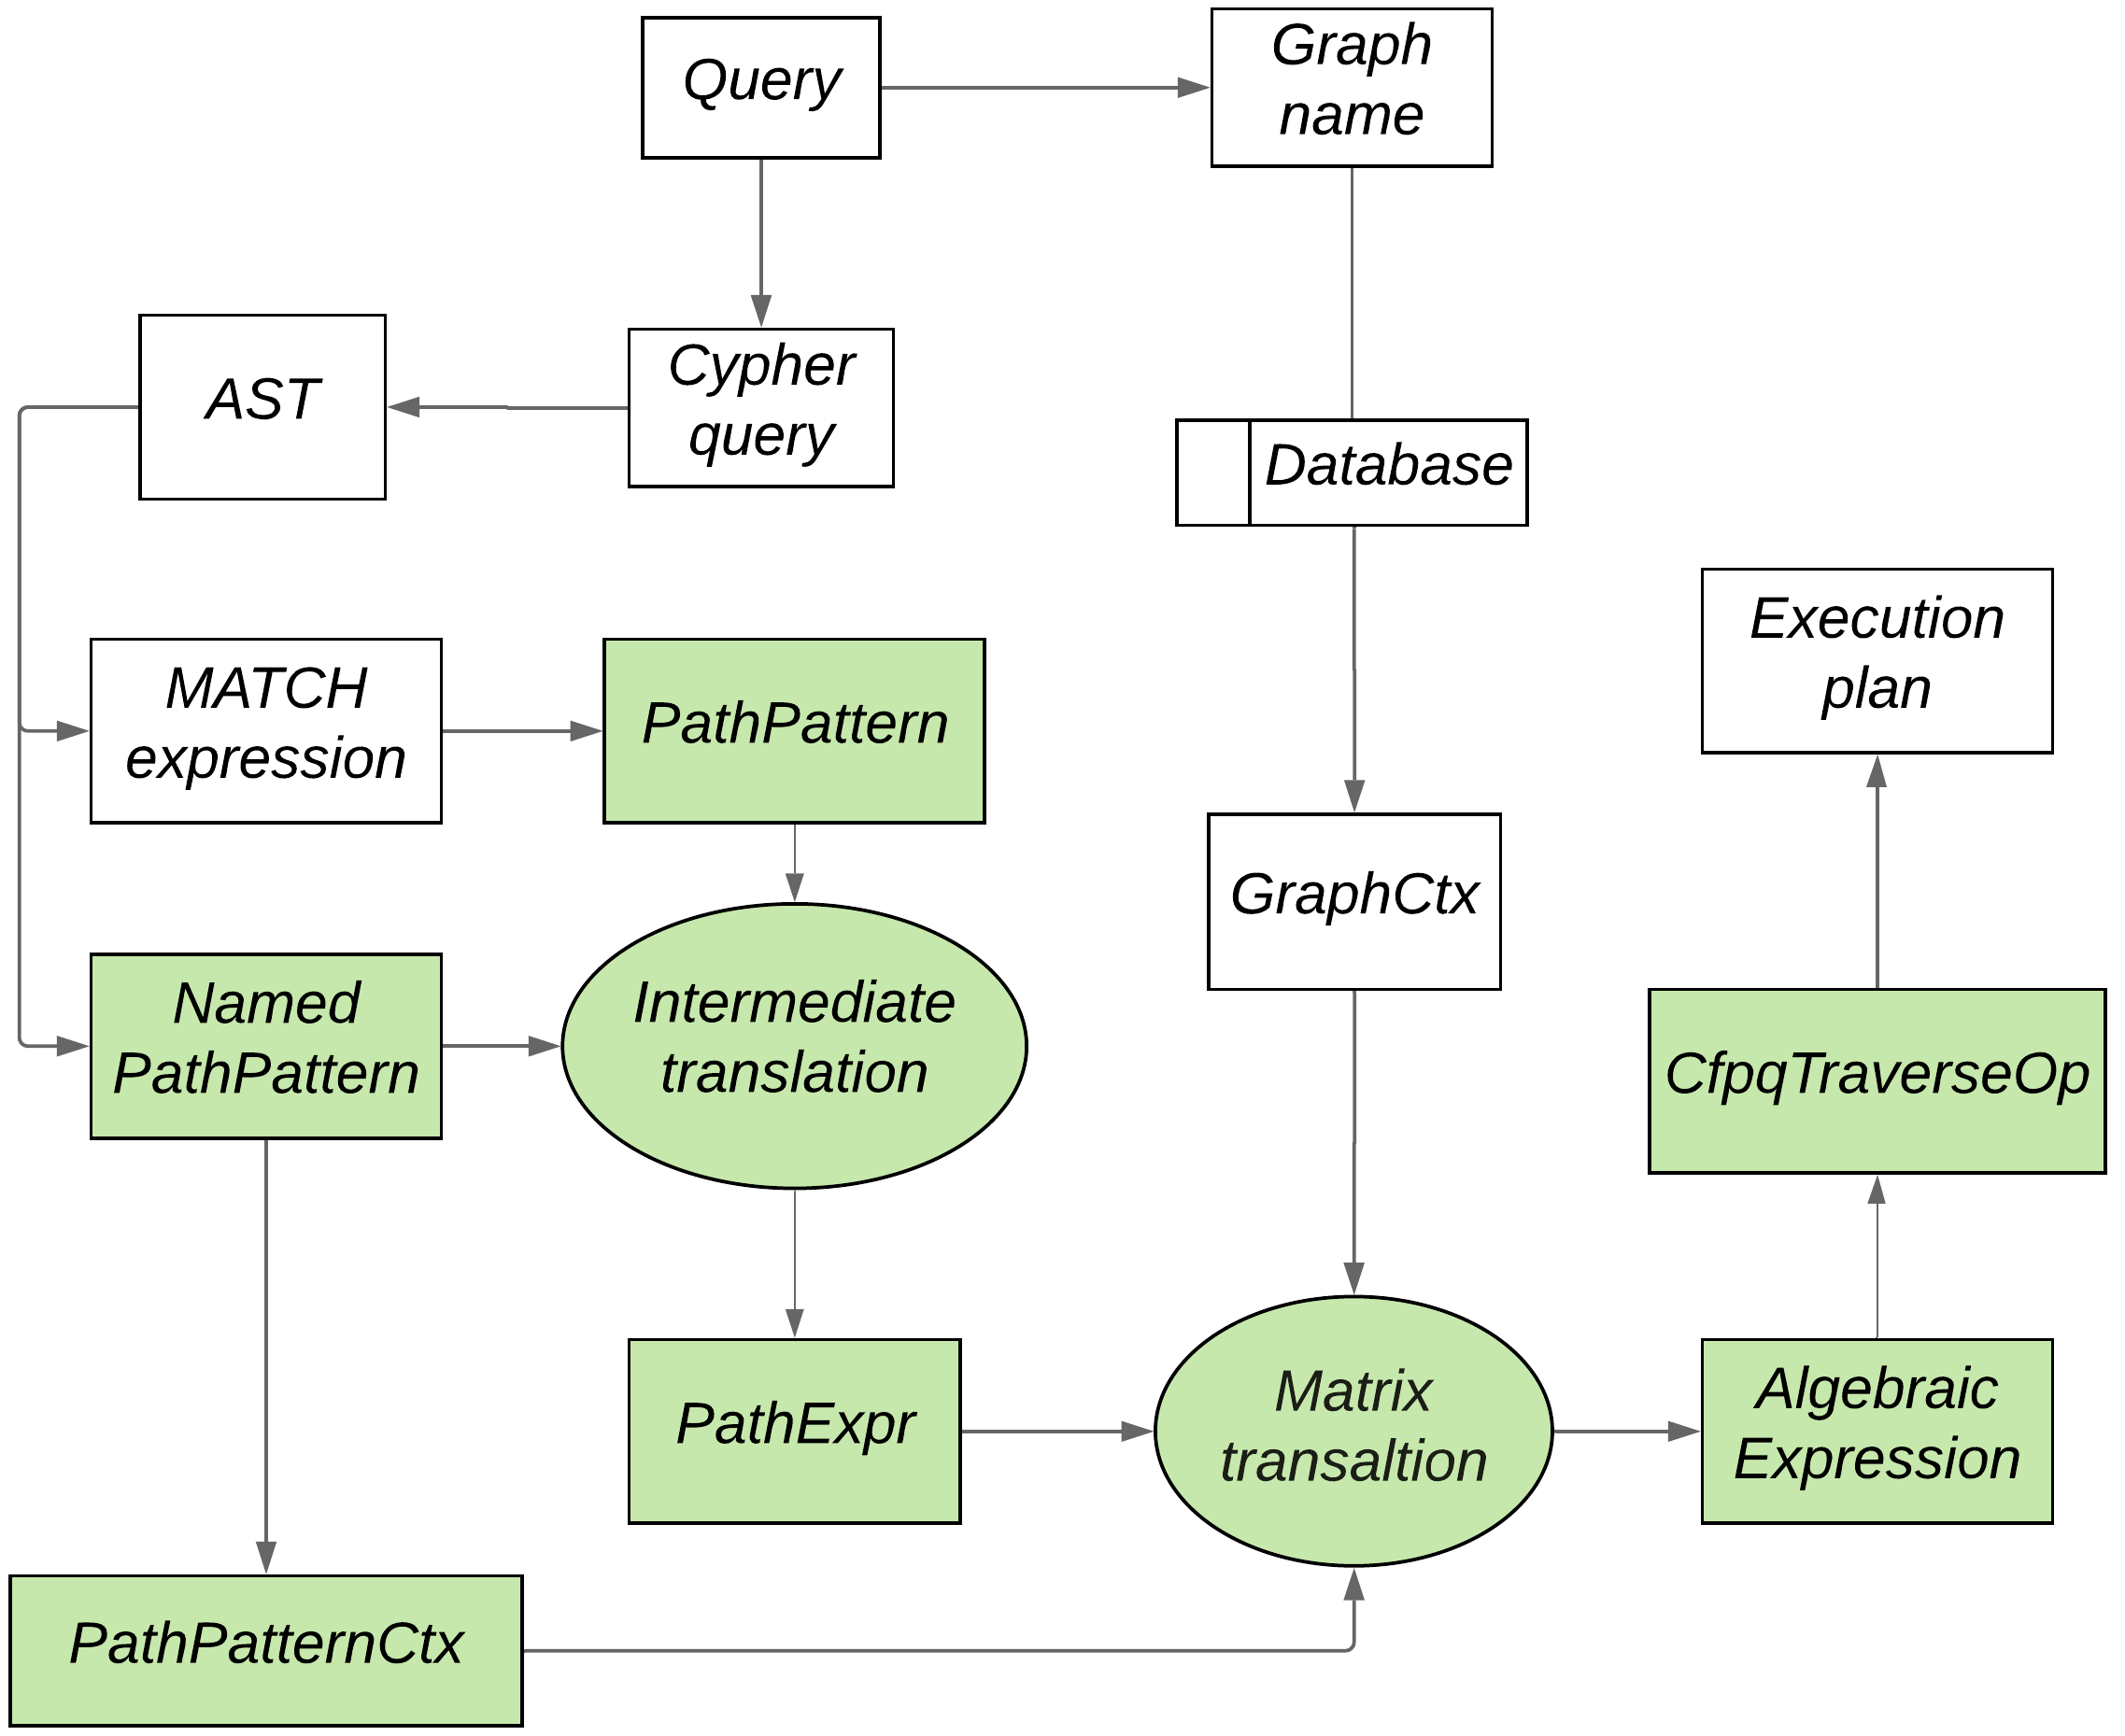
\includegraphics[width=1.0\linewidth]{Terekhov/pictures/execution_plan_3.png}
    \caption{Расширение построения плана выполнения запроса}
    \label{fig:execution_plan}
\end{figure}

\subsection{Промежуточное представление}\label{matrix-translation}
Шаблоны путей, полученные из \textit{AST}, транслируются в промежуточное представление \textit{PathExpr}. Оно позволяет задавать более простой абстрактный синтаксис, который описан на рисунке~\ref{fig:intermidiate_repr}. 

Таким образом, альтернативе и конкатенации шаблонов соответствуют \textit{PathAlt} и \textit{PathSeq}, \textit{PathGroup} позволяет задавать направление пути и наличие замыкания, а \textit{PathBasic} соответствует либо примитивным шаблонам \textit{PathNode}, \textit{PathEdge} и \textit{PathRef}, либо целому выражению \textit{PathExpr}. Примеры промежуточного представления шаблонов приведены в таблице~\ref{tab:inter_examples}.
\begin{figure}[h!]
\begin{align*}
\begin{split}
PathExpr=~ &PathSeq(PathExpr,~PathExpr)~|\\
           &PathAlt(PathExpr,~PathExpr)~|\\
           &PathGroup(PathBasic, direction, range)
\end{split}\\
\begin{split}
PathBasic=~ &PathNode(label)~|\\
            &PathEdge(type)~~|\\
            &PathRef(name) ~~|\\
            &PathExpr
\end{split}\\
\begin{split}
direction \in ~&\{inbound,~outbound,~bidirectional\}\\
range \in     ~&\{*, \varnothing\}
\end{split}
\end{align*}
\caption{Промежуточное представление PathExpr}
\label{fig:intermidiate_repr}
\end{figure}

\begin{table}[h]
\centering
\begin{adjustbox}{max width=\textwidth}
\begin{tabular}{|c|l|}
\hline
$L_p$                        & \multicolumn{1}{c|}{PathExpr}                                                                                                        \\ \hline
{[}:A :B{]} | (:C)           & \begin{tabular}[c]{@{}l@{}}$PathAlt($\\ $~~~~PathSeq(PathEdge("A"),~PathEdge("B"))$\\ $~~~~PathNode("C")$\\ $)$\end{tabular}         \\ \hline
\textless{}{[}:A $\sim$S{]}* & \begin{tabular}[c]{@{}l@{}}$PathGroup($\\ $~~~~PathSeq(PathEdge("A"),~PathRef("S")),$\\ $~~~~inbound,$\\ $~~~~*,$\\ $)$\end{tabular} \\ \hline
\end{tabular}
\end{adjustbox}
\caption{Примеры промежуточного представления запросов}
\label{tab:inter_examples}
\end{table}

\newpage
\subsection{Трансляция в матричные выражения}
Как было упомянуто ранее, RedisGraph представляет графы в виде разреженных матриц. А именно каждый граф $G$ задаётся следующей тройкой $(A \in M_{n\times n},~lab \in Labels \rightarrow Diag_n,~rel \in RelTypes \rightarrow M_{n \times n})_G$. Здесь $M_{n \times n}$ означает полукольцо булевых матриц, а $Diag_n$ полукольцо диагональных булевых матриц. Матрица $A$ служит матрицей смежности графа, а отображения $lab$ и $rel$ сопоставляют меткам вершин и типам рёбер соответствующие булевы матрицы. Таким образом, ребро $(v, to)$ графа $G$ имеет тип $a$ тогда и только тогда, когда $rel(a)_{v,to} = 1$.  Таким же образом, принадлежность метки $l$ вершине $v$ равносильно $lab(l)_{v,v}=1$.

Любую булеву матрицу $M$, участвующую в задании графа $G(V, E)$, можно рассматривать как отношение на множестве вершин $R(M) = \{(v, to):~M_{v,to}=1\}$. Операциями сложения и умножения в булевом полукольце являются дизъюнкция и конъюнкция. Поэтому умножению матриц $A*B$ соответствует композиция отношений $R(A) \circ R(B)$, сложению $A+B$ соответствует объединение отношений $R(A) \cup R(B)$, а транспонированная матрица $A^T$ соответствует обратному к R(A) отношению $R(A)^{-1}$. Такая взаимосвязь между матричными операциями и отношениями лежит в основе алгоритма трансляции, приведённом на рисунке~\ref{algo:translation}.

Данный алгоритм является рекурсивным и принимает на вход промежуточное представление шаблона пути $expr$, представление графа $g$ и контекст именованных шаблонов путей $pathCtx$. Целевым языком трансляции является простой язык матричных выражений, приведённый на рисунке~\ref{fig:alg-expr}.

Базовым случаем рекурсии являются примитивные шаблоны \textit{Path\-Node}, \textit{PathEdge} и \textit{PathReference}, которые транслируются в операнды матричного выражения. Для первых двух соответствующие матрицы извлекаются из графа с помощью функций \textit{GetLabel\-Matrix} и \textit{GetRelation\-Matrix}. При этом случай $label = \varnothing$ соответствует шаблону пути, состоящему из одной произвольной вершины. Поэтому такой путь задаётся тождественным отношением $R(I)$, где $I$ --- единичная матрица. Для \textit{Path\-Reference} создаётся ссылка на матрицу именованного шаблона, которая будет вычислена на следующем этапе при выполнении алгоритма контекстно-свободной достижимости.

Трансляция для шаблонов \textit{PathSeq} и \textit{PathAlt} происходит одинаковым образом --- сначала происходит трансляция дочерних шаблонов, а потом из полученного результата образуются операции умножения или сложения. Такая трансляция обосновывается семантикой шаблонов альтернативы и конкатенации, приведенной в главе~\ref{subsection:cypher-extention}, и связью отношений с матричными операциями, описанными раннее.

Наиболее интересным случаем является трансляция \textit{Path\-Group}, так как в некоторых случаях контекст именованных шаблонов $pathCtx$ расширяется. В начале происходит трансляция дочернего шаблона. Далее, если заданное направление является обратным, к полученной матрице применяется операция транспонирования. Если же направление является произвольным, то формируется операция сложения из полученной матрицы и транспонированной к ней. Это соответствует альтернативе между прямым путём и обратным к нему. После этого при отсутствии замыкания результат возвращается. Иначе происходит трансляция замыкания полученного выражения. Так как его нельзя выразить через имеющиеся матричные операции, создаётся новый именованный шаблон, а замыкание заменяется ссылкой на него. Нетрудно показать, что регулярное выражение $R^*$ и контекстно-свободная грамматика с одним правилом $S \rightarrow R~S \mid \epsilon$ равносильны. Поэтому правая часть этого правила тривиальным образом сразу же транслируется в выражение \textit{Add(Mul(R, MatrixRef(S)), I)} и добавляется в \textit{pathCtx} вместе с полученным новым именем.

Таким образом, после работы данного алгоритма из промежуточного представления шаблона пути получается выражение над матрицами. При дальнейшем его вычислении получается матрица, которая соответствует такому же отношению на множестве вершин, как и семантика изначального шаблона.

\algnewcommand\algorithmicswitch{\textbf{switch}}
\algnewcommand\algorithmiccase{\textbf{case}}
\algnewcommand\algorithmicof{\textbf{of}}
\algnewcommand\algorithmicassert{\texttt{assert}}
\algnewcommand\algorithmiccasepart{\texttt{:}}
\algnewcommand\Assert[1]{\State \algorithmicassert(#1)}%
% New "environments"
\algdef{SE}[SWITCH]{Switch}{EndSwitch}[1]{\algorithmicswitch\ #1}{\algorithmicend\ \algorithmicswitch}%
\algdef{SE}[CASE]{Case}{EndCase}[1]{\algorithmiccase\ #1\algorithmiccasepart}{\algorithmicend\ \algorithmiccase}%
\algdef{SE}[CASEPART]{CasePart}{EndCasePart}[1]{#1\algorithmiccasepart}{\algorithmicend\ \algorithmiccasepart}%
\algtext*{EndSwitch}%
\algtext*{EndCase}%
\algtext*{EndCasePart}%

\begin{algorithm}
\caption{Алгоритм трансляции}
\begin{algorithmic}[1]
\Function{translate}{PathExpr expr, GraphCtx g, PathPatternCtx pathCtx}
    \Switch{expr}
        \Case{$PathNode$(label)}
            \If{label $== \varnothing$}
                \State \Return \Call{GetIdentityMatrix}{g}
            \Else
                \State \Return \Call{GetLabelMatrix}{g, label}
            \EndIf
        \EndCase
        \Case{$PathEdge$(type)}
            \State \Return \Call{GetRelationMatrix}{g, type}
        \EndCase
        \Case{$PathRef(name)$}
            \State \Return $MatrixRef$(name)
        \EndCase
        \Case{$PathSeq$(left, right)}
            \State \Return Add(\Call{translate}{left}, \Call{translate}{right})
        \EndCase
        \Case{$PathAlt$(left, right)}
            \State \Return Mul(\Call{translate}{left}, \Call{translate}{right})
        \EndCase
        \Case{$PathGroup$(basic, dir, range)}
            \State res = \Call{translte}{basic}
            \Switch{dir}
                \Case{$inbound$}
                    \State res = $Transpose$(res)
                \EndCase
                \Case{$bidirectional$}
                    \State res = $Add$(res, $Transpose$(res))
                \EndCase
            \EndSwitch
            \Switch{range}
                \Case{ $\varnothing$}
                    \State \Return res
                \EndCase
                \Case{$*$}
                    \State name = \Call{AllocateNewPathPattern}{ctx}
                    \State res = $Mul$(res, $MatrixRef$(name))
                    \State res = $Add$(res, \Call{GetIdentityMatrix}{g})
                    \State \Call{SetPathPetternExpression}{p, name, res}
                    \State \Return $MatrixRef$(name)
                \EndCase
            \EndSwitch
        \EndCase
    \EndSwitch
\EndFunction
\end{algorithmic}
\caption{Алгоритм транслции в матричные выражения}
\label{algo:translation}
\end{algorithm}

\begin{figure}[H]
\begin{align*}
\begin{split}
AlgExpr= ~ &Add(AlgExpr, AlgExpr)~|\\
           &Mul(AlgExpr, AlgExpr)~|\\
           &Transpose(AlgExpr)~|\\
           &Matrix~|\\
           &MatrixRef(ref)
\end{split}
\end{align*}
\caption{Алгебраическое выражение над матрицами}
\label{fig:alg-expr}
\end{figure}

\subsection{Формирование и вычисление операции плана выполнения}
После этапа трансляции в RedisGraph происходит построение плана выполнения запроса. Он формируется из последовательности операций, которые выполняют базовые вычисления. Для поддержки шаблонов путей была добавлена операция \textit{CfpqTraverseOp}. Она создаётся для каждого матричного выражения, полученного на предыдущем шаге из неименованого шаблона пути, и отвечает за его вычисление.

На этапе инициализации новой операции \textit{CfpqTraverseOp} из соответствующего матричного выражения рекурсивно извлекаются все ссылки на именованные шаблоны путей, от которых зависит данное выражение. После этого они поступают на вход алгоритма, решающего задачу контекстно-свободной достижимости (см. алгоритм 4).

Этот алгоритм является расширенной версией матричного алгоритма Рустама Азимова, приведенного в главе~\ref{sec:matrix-algo}. В данном алгоритме, в отличие от алгоритма Рустама Азимова, не требуется задавать правила грамматики в ослабленной нормальной форме Хомского. Вместо этого правая часть правила задаётся с помощью промежуточного представления \textit{PathExpr}. При этом подразумевается, что для любого именованного шаблона $p$ из глобального контекста \textit{pathCtx} его промежуточное представление уже транслировано в матричное выражение и записано в \textit{pathCtx[p].algExpr}.

Принцип работы алгоритма остаётся прежним. На каждой итерации для всех невычисленных шаблонов происходит вычисление матричного выражения. Если результирующая матрица не изменяется, то она является окончательной для данного именованного шаблона и он больше не участвует в обновлении. Иначе соответствующая матрица перезаписывается.

После работы данного алгоритма все ссылки на именованные шаблоны путей в матричном выражении заменяются на подсчитанные алгоритмом матрицы, после чего происходит вычисление матричного выражения. Результат сохраняется в операции $CfpqTraverseOp$ и участвует в вычислении плана выполнения запроса наряду с результатами других операций. 
\begin{algorithm}
\begin{algorithmic}[1]
\Function{CfpqTraverseNew}{String[] patterns, PathPatternCtx pathCtx}
\While{$\exists$ p $\in$ patterns: !pathCtx[p].isEvaluated}
    \ForAll{p $\in$ patterns}
        \If{!pathCtx[p].isEvaluated}
            \State new\_matrix = \Call{EvalueteAlgExpr}{pathCtx[p].expr}
            \If{new\_matrix == pathCtx[p].matrix}
                \State pathCtx[p].isEvaluated = true
            \Else
                \State pathCtx[p].matrix = new\_matrix
            \EndIf
        \EndIf
    \EndFor
\EndWhile
\EndFunction
\end{algorithmic}
\label{algo:matrix-extention}
\caption{Расширенный матричный алгоритм}
\end{algorithm}


\section{Замеры производительности}
После реализации поддержки нового синтаксиса шаблонов путей были произведены замеры производительности.

\subsection{Сравнение с парсер-комбинаторами}\label{sec:parse-comp-compare}
Сравнительный анализ времени работы полученного решения (колонка RedisGraph) и библиотеки парсер-комбинаторов (колонка Meer\-kat), описанной в главе~\ref{sec:pareser-combinators}, приведён в таблице~\ref{tab:combinators-vs-redisgraph}. Запросы были взяты из эксперимента оригинальной статьи про парсер-комбинаторы~\cite{parser-combinators}. Эквивалентные им запросы, написанные в расширенном синтаксисе Cyp\-her, приведены на рисунках~\ref{code:sub_clas_of_1},~\ref{code:sub_clas_of_2} и представляют из себя частный случай запросов поиска объектов, лежащих на одном уровне иерархии. Набор графов также был взят из вышеупомянутого эксперимента и впервые был представлен в статье Сяованга Чжана~\cite{zhlang-2016}.

% \gsv{У Вас в тексте минимум два разных варианта написания названия этой библиотеки. Надо бы узнать, как правильно и унифицировать}
% \gsv{ лежащих на одном уровне в иерархии}

Замеры обоих решений производились локально на оборудовании со следующими характеристиками: Intel Core i7 4$\times$1.8GHz, 8 GB RAM. Каждый запрос запускался 20 раз и время его работы усреднялось. Время работы указано в миллисекундах. Также в колонках $|V|$ и $|E|$ указано количество вершин и рёбер графа, а в колонке $\#result$ количество найденных соответствующим запросом пар вершин. 

\begin{table}[h!]
\begin{adjustbox}{max width=\textwidth}
\begin{tabular}{|l|c|c|c|c|c|c|c|c|}
\hline
\multicolumn{1}{|c|}{\multirow{2}{*}{$G$}}                   & \multirow{2}{*}{$|V|$} & \multirow{2}{*}{$|E|$} & \multicolumn{3}{c|}{Query\_1}                                                                                                           & \multicolumn{3}{c|}{Query\_2}                                                                                                           \\ \cline{4-9} 
\multicolumn{1}{|c|}{}                                       &                        &                        & \#result & \begin{tabular}[c]{@{}c@{}}Meerkat\\ time (ms)\end{tabular} & \begin{tabular}[c]{@{}c@{}}RedisGraph\\ time (ms)\end{tabular} & \#result & \begin{tabular}[c]{@{}c@{}}Meerkat\\ time (ms)\end{tabular} & \begin{tabular}[c]{@{}c@{}}RedisGraph\\ time (ms)\end{tabular} \\ \hline
wine                                                         & 773                    & 2450                   & 66572    & 541                                                         & 31                                                             & 133      & 6                                                           & 3                                                              \\ \hline
pizza                                                        & 671                    & 2604                   & 56195    & 476                                                         & 24                                                             & 1262     & 30                                                          & 4                                                              \\ \hline
\begin{tabular}[c]{@{}l@{}}measure-\\ primitive\end{tabular} & 341                    & 771                    & 15156    & 158                                                         & 11                                                             & 2871     & 39                                                          & 5                                                              \\ \hline
funding                                                      & 778                    & 1480                   & 17634    & 99                                                          & 14                                                             & 1158     & 14                                                          & 6                                                              \\ \hline
\begin{tabular}[c]{@{}l@{}}atom-\\ primitive\end{tabular}    & 291                    & 685                    & 15454    & 102                                                         & 10                                                             & 122      & 53                                                          & 3                                                              \\ \hline
\begin{tabular}[c]{@{}l@{}}people-\\ pets\end{tabular}       & 337                    & 834                    & 9472     & 55                                                          & 7                                                              & 37       & 3                                                           & 3                                                              \\ \hline
travel                                                       & 131                    & 397                    & 2449     & 21                                                          & 3                                                              & 63       & 2                                                           & 2                                                              \\ \hline
\end{tabular}
\end{adjustbox}
\caption{Сравнение Meerkat и полученного решения}
\label{tab:combinators-vs-redisgraph}
\end{table}

\begin{figure}[h!]
\begin{adjustbox}{max width=\textwidth}
\begin{lstlisting}[language=sql]
PATH PATTERN S = ()-/ [<:Type     [~S | ()] :Type] | 
                      [<:SubClass [~S | ()] :SubClass] /-()
MATCH (v)-/ ~S /->(to)
RETURN COUNT(*)
\end{lstlisting}
\end{adjustbox}
\caption{Query\_1}
\label{code:sub_clas_of_1}
\end{figure}

\begin{figure}[h!]
\begin{adjustbox}{max width=\textwidth}
\begin{lstlisting}[language=sql]
PATH PATTERN S = ()-/ :SubClass | [<:SubClass ~S :SubClass] /-()
MATCH (v)-/ ~S /->(to)
RETURN COUNT(*)
\end{lstlisting}
\end{adjustbox}
\caption{Query\_2}
\label{code:sub_clas_of_2}
\end{figure}

По результатам замеров видно, что даже на небольших графах время работы Meerkat сильно больше, чем время работы полученного решения. При этом в большинстве случаев оно отличатся на порядок. Также стоит отметить, что запросы, указанные на рисунках~\ref{code:sub_clas_of_1},~\ref{code:sub_clas_of_2}, помимо расширенного синтаксиса используют и оригинальную часть языка Cyp\-her, а конкретно функцию COUNT. Это является небольшим примером того, что расширение языка запросов является полностью совместимым с его оригинальной частью.

% Эксперимент, проведенный в статье про парсер-комбинаторы, описанные в  был повторён локально на оборудовании с характеристиками.
% Каждое матричное выражение, полученное при трансляции шаблонов путей, формирует операцию плана выполнения запроса $CfpqTraverse$.

\subsection{Сравнение с матричным алгоритмом}
Графы, приведенные в предыдущих замерах являются достаточно маленькими, поэтому также были произведены замеры на более больших графах. Они были взяты из набора данных CFPQ\_Data~\cite{cfpq-data}, собранного исследователями лаборатории языков инструментов JetBrains Research. Замеры производились таким же образом и на том же оборудовании, что и в главе~\ref{sec:parse-comp-compare}.

% \gsv{Кажется, что нет. go  и прочие большие графы уже просто из нашего набора данных CFPQ\_Data, у китайцев их не было.}

Кроме этого, для анализа издержек выполнения запроса в таблице~\ref{tab:combinators_vs_redisgraph} приводится время работы оригинального алгоритма Рустама Азимова (колонка Matrix algorithm), описанного в главе~\ref{sec:matrix-algo}. Данный алгоритм был интегрирован в RedisGraph и запускался на графах, находящихся в его хранилище. Для этого была разработана отдельная команда, принимающая на вход название графа и путь до файла с грамматикой, написанной в нормальной форме Хомского. Для вычисления матричных операций также использовалась библиотека SuiteSparse.

Таким образом, во-первых, время работы оригинального алгоритма не включает в себя издержки, возникающие при выполнении запроса внутри графовой базы данных. Во-вторых, оригинальный алгоритм отличается от алгоритма, используемого при выполнении запроса в расширенном синтаксисе. Тем не менее время работы обоих решений отличается не сильно и является достаточно небольшим для применения на практике.
\begin{table}[h!]
\begin{adjustbox}{max width=\textwidth}
\begin{tabular}{|l|c|c|c|c|c|c|c|c|}
\hline
\multicolumn{1}{|c|}{\multirow{2}{*}{$G$}} & \multirow{2}{*}{$|V|$} & \multirow{2}{*}{$|E|$} & \multicolumn{3}{c|}{Query\_1}                                                                                                                      & \multicolumn{3}{c|}{Query\_2}                                                                                                                      \\ \cline{4-9} 
\multicolumn{1}{|c|}{}                     &                        &                        & \#result & \begin{tabular}[c]{@{}c@{}}Matrix\\ algorithm\\ time (ms)\end{tabular} & \begin{tabular}[c]{@{}c@{}}RedisGraph\\ time (ms)\end{tabular} & \#result & \begin{tabular}[c]{@{}c@{}}Matrix\\ algorithm\\ time (ms)\end{tabular} & \begin{tabular}[c]{@{}c@{}}RedisGraph\\ time (ms)\end{tabular} \\ \hline
go                                         & 272770                 & 1068622                & 304070   & 1272                                                                   & 1236                                                           & 334850   & 662                                                                    & 683                                                            \\ \hline
go-hierarchy                               & 45007                  & 1960436                & 588976   & 271                                                                    & 276                                                            & 738937   & 193                                                                    & 290                                                            \\ \hline
eclass-514                                 & 48815                  & 219390                 & 90994    & 198                                                                    & 304                                                            & 96163    & 121                                                                    & 241                                                            \\ \hline
enzyme                                     & 239111                 & 1047454                & 396      & 103                                                                    & 47                                                             & 8163     & 68                                                                     & 37                                                             \\ \hline
\end{tabular}
\end{adjustbox}
\caption{Сравнение матричного алгоритма и полученного решения}
\label{tab:combinators_vs_redisgraph}
\end{table}

\subsection{Сравнение с анализом Йохема Куйперса}
Также был произведён замер времени работы на очень большом графе geospeices~\cite{geospices}. Этот граф является довольно важным, потому что он участвовал в сравнительном анализе алгоритмов, проведенным Йохемом Куйперсом. Именно из-за колоссального времени работы запроса на данном графе дальнейшее расширение языка запросов Йохемом Куйперсом и др. было приостановлено. 

Повторить эксперимент не предоставилось возможным, так как в статье не приводились ссылки на реализацию алгоритмов. Поэтому в таблице~\ref{tab:neo4j-vs-redisgraph} приводится замер из оригинальной статьи алгоритма с наилучшим временем работы (колонка Neo4j). Время указано в секундах. Эквивалентный запрос в расширенном синтаксисе приводится на рисунке~\ref{code:broaderTransitive}. Характеристики оборудования, на которых выполнялись запросы, следующие:

\begin{itemize}
    \item Neo4j: Intel Xeon E5-4610 v2, 8$\times$2.30GHz, 400 GB RAM
    \item RedisGraph: Intel Core i7-6700 CPU, 64 GB RAM 4$\times$3.4GHz
\end{itemize}

\begin{figure}[h!]
\begin{adjustbox}{max width=\textwidth}
\begin{lstlisting}[language=sql]
PATH PATTERN S = ()-/ [:broaderTransitive [~S | ()] <:broaderTransitive] /-()
MATCH (v)-/ ~S /->(to)
RETURN COUNT(*)
\end{lstlisting}
\end{adjustbox}
\caption{Query}
\label{code:broaderTransitive}
\end{figure}

\begin{table}[h!]
\begin{adjustbox}{max width=\textwidth}
\begin{tabular}{|l|c|c|c|c|c|}
\hline
\multicolumn{1}{|c|}{G} & $|V|$   & $|E|$     & \#result    & \begin{tabular}[c]{@{}c@{}}Neo4j\\ time (s)\end{tabular} & \begin{tabular}[c]{@{}c@{}}RedisGraph\\ time (s)\end{tabular} \\ \hline
geospeices              & 225 000 & 1 550 000 & 226 669 749 & 6 953.9                                                       & 26.1                                                          \\ \hline
\end{tabular}
\end{adjustbox}
\caption{Сравнение с замером Йохема Куйперса}
\label{tab:neo4j-vs-redisgraph}
\end{table}

По результатам замеров видно, что удалось достичь времени работы в десятки секунд. Такое время было обозначено Куйперсом как приемлемое время работы для практического применения.

% \gsv{а значит .... Закончите мысль выводом.} 

\subsection{Выводы}
По результатам замеров времени выполнения можно говорить о том, что полученное решение делает запросы с контекстно-свободными ограничениями доступными для практического применения. При этом новый синтаксис языка сильно расширяет его возможности и является полностью совместимым с его оригинальной версией.

\section*{Заключение}
В ходе работы были получены следующие результаты:
\begin{itemize}
\item Выполнен обзор текущих решений поддержки запросов с кон\-текстно-свободными ограничениями, по результатам которого было решено интегрировать матричный алгоритм Рустама Азимова в графовую базу данных RedisGraph с последующим расширением языка запросов Cypher. 
\item Интегрирован матричный алгоритм Рустама Азимова в RedisGraph.
\item Разработана поддержка расширения языка запросов Cypher для RedisGraph, позволяющая задавать запросы с конте\-кстно-сво\-бод\-ными ограничениями. Исходный код находится в репозитории на github~\cite{github}. Также для удобства и возможности позапускать запросы без процесса установки необходимого программного обеспечения предоставляется docker контейнер~\cite{docker}.
\item Произведены замеры производительности полученного решения и сравнение времени работы с текущими аналогами.
\item Результаты работы изложены в статье, принятой на конференцию GRADES-NDA 2020.
\end{itemize}

В будущем планируется разработать подробную пользовательскую документацию запросов в расширенном синтаксисе, так как черновой вариант официальной спецификации рассчитан больше на разработчиков. Также планируется отправить запрос на принятие изменений в официальный репозиторий RedisGraph. 

%\setmonofont[Mapping=tex-text]{CMU Typewriter Text}
%\bibliographystyle{ugost2008ls}
%\bibliography{diploma.bib}
%\end{document}

\newcommand\dictionaryct
{
\begin{multicols}{2}
    \begin{lstlisting}
interface (*\ienumerable*) {}
interface (*\icollectiontype:*) (*\ienumerable*) {}
interface (*\ienumerable\texttt{<}*)out(*~\xtype\texttt{>}:*)
    (*\ienumerable*){}
struct (*\keyvaluepairtype\texttt{<}\xtype, \ytype\texttt{>}*) {}
interface (*\onector{\icollectiontype}{\xtype}:*)
    (*\onector{\ienumerable}{\xtype}*) {}
interface (*\idictionarytype:*) (*\icollectiontype*) {}
interface (*\onector{\idictionarytype}{\xtype, \ytype}:*)
    (*\onector{\icollectiontype}{\onector{\keyvaluepairtype}{\xtype, \ytype}}*) {}
class (*\onector{\dictionarytype}{\xtype, \ytype}:*)
    (*\onector{\idictionarytype}{\xtype, \ytype}*),
    (*\idictionarytype*) {}
    \end{lstlisting}
    \columnbreak
    \begin{alignat*}{3}
        \classtableline{\objecttype}{} \\
        \classtableline{\valuetype}{\objecttype} \\
        \classtableline{\ienumerable}{\objecttype} \\
        \classtableline{\onector{\ienumerable}{+\xtype}}{\ienumerable} \\
        \classtableline{\onector{\keyvaluepairtype}{\xtype, \ytype}}{\valuetype} \\
        \classtableline{\icollectiontype}{\ienumerable} \\
        \classtableline{\onector{\icollectiontype}{\xtype}}{\onector{\ienumerable}{\xtype}} \\
        \classtableline{\onector{\idictionarytype}{\xtype, \ytype}}{\onector{\icollectiontype}{\onector{\keyvaluepairtype}{\xtype, \ytype}}} \\
        \classtableline{\onector{\dictionarytype}{\xtype, \ytype}}{\onector{\idictionarytype}{\xtype, \ytype}} \\
        \addclasstableline{\idictionarytype}
    \end{alignat*}
\end{multicols}
}

\newcommand\pcpct
{
    \begin{alignat*}{3}%
        \classtableline{\onector{\pcpfstsym}{+\pcpxtype}}{} \\
        &&\vdots \\
        \classtableline{\onector{\pcpsndsym}{+\pcpxtype}}{} \\
        \classtableline{\onector{\pcprconstr}{+\pcpxtype}}{} \\
        \classtableline{\onector{\pcpsconstr}{+\pcpxtype}}{} \\
        \classtableline{\pcprconstr_{0}}{\pcprconstr\pcprconstr_{0}, \, \pcpeconstr} \\
        \classtableline{\pcpsconstr_{0}}{\pcpsconstr\pcpsconstr_{0}, \, \pcpeconstr} \\
        \classtableline{\pcpeconstr}{} \\
        \classtableline{\onector{\pcpuword{1}}{+\pcpxtype}}{\overline{\pcpuword{1}}\pcpxtype, \, \pcpwword{1}\pcpxtype, \, \pcpsconstr\pcpxtype, \, \pcprconstr\pcpxtype} \\
        &&\vdots \\
        \classtableline{\onector{\pcpuword{n}}{+\pcpxtype}}{\overline{\pcpuword{n}}\pcpxtype, \, \pcpwword{n}\pcpxtype,  \, \pcpsconstr\pcpxtype, \, \pcprconstr\pcpxtype} \\
        \classtableline{\onector{\pcpvword{1}}{+\pcpytype}}{\overline{\pcpvword{1}}\pcpytype, \, \pcpwword{1}\pcpytype,  \, \pcpsconstr\pcpytype, \, \pcprconstr\pcpytype} \\
        &&\vdots \\
        \classtableline{\onector{\pcpvword{n}}{+\pcpytype}}{\overline{\pcpvword{n}}\pcpytype, \, \pcpwword{n}\pcpytype,  \, \pcpsconstr\pcpytype, \, \pcprconstr\pcpytype} \\
        \classtableline{\onector{\pcpwword{1}}{+\pcpxtype}}{} \\
        &&\vdots \\
        \classtableline{\onector{\pcpwword{n}}{+\pcpxtype}}{} \\
        \classtableline{\pcprestalt}{\pcpuword{1}\pcprestalt, \ldots, \pcpuword{n}\pcprestalt, \, \pcpeconstr} \\
        \classtableline{\pcprestblt}{\pcpvword{1}\pcprestblt, \ldots, \pcpvword{n}\pcprestblt, \, \pcpeconstr} \\
        \classtableline{\pcprestart}{\pcpuword{1}\pcprestart, \ldots, \pcpuword{n}\pcprestart, \, \pcpeconstr} \\
        \classtableline{\pcprestbrt}{\pcpvword{1}\pcprestbrt, \ldots, \pcpvword{n}\pcprestbrt, \, \pcpeconstr} \\
        \classtableline{\pcprestct}{\pcpwword{1}\pcprestct, \ldots, \pcpwword{n}\pcprestct,\, \pcpeconstr} \\
        \classtableline{\pcpdword}{\overline{\pcpuword{1}}\pcpdword,\ldots, \overline{\pcpuword{n}}\pcpdword, \, \pcpeconstr} \\
    \end{alignat*}%
}

\section{Система типов\protect\footnotemark}
\footnotetext{Эта глава частично повторяет описание системы типов из работы~\cite{kennedy2006decidability}.}

В этой главе мы формализуем номинальное подтипирования с вариантностью. Типы могут быть либо типовыми переменными, обозначаемыми строчными буквами, или сконструированными типами $\ctor{C}{T}$, где $C$ является $n$-арным типовым конструктором, а $\overline{T}$ --- вектором из аргументов длины $n$. Если типовой конструктор является унарным, мы будем опускать угловые скобки: например, мы будем писать $ABCx$ вместо $\onector{A}{\onector{B}{\onector{C}{x}}}$. $C^{r}T$ обозначает $C\ldots CT$, где $C$ появляется $r$ раз. Мы рассматриваем такие типы как последовательность из $r$ типовых конструкторов $C$, закачивающеюся типом $T$. \emph{Закрытыми} типами будем называть типы, которые не содержат типовых переменных. \emph{Открытыми} типами будем называть не закрытые типы.

Отношение подтипирования в номинальных системах типов с вариантностью определяется явно указанием имён надтипов и \emph{вариантностями} типовых параметров, и обычно представляются таблицей классов.

\begin{defn}
\emph{Таблица классов} --- это конечное множество записей следующего вида
\generalclasstable{\ctor{C}{\vvariance x}}{T}{n}{}

Каждая запись содержит уникальное описание типового конструктора и конечный список сконструированных типов. Типы из списка являются номинальными надтипами для всех типов, которые будут сконструированы соответствующим типовым конструктором. Левая часть записи содержит имя конструктора $C$ и его формальные типовые параметры $x_{i}$ с \emph{вариантностями} $\vvariance_i$. \(\vvariance_i\) может быть либо \(\circ\)~(инвариантность), или \(+\)~(ковариантность), или \(-\)~(контравариантность). Для упрощения нотации будем опускать $\circ$ в определении таблицы классов.
\end{defn}

\begin{Listing}
\small{    \begin{lstlisting}
interface (*\ienumerable*) {}
interface (*\ienumerable\texttt{<}*)out(*~\xtype\texttt{>}:*)
    (*\ienumerable*){}
interface (*\icollectiontype:*) (*\ienumerable*) {}
interface (*\onector{\icollectiontype}{\xtype}:*)
    (*\onector{\ienumerable}{\xtype}*) {}
struct (*\keyvaluepairtype\texttt{<}\xtype, \ytype\texttt{>}*) {}
interface (*\idictionarytype:*) (*\icollectiontype*) {}
interface (*\onector{\idictionarytype}{\xtype, \ytype}:*)
    (*\onector{\icollectiontype}{\onector{\keyvaluepairtype}{\xtype, \ytype}}*) {}
class (*\onector{\dictionarytype}{\xtype, \ytype}:*)
    (*\onector{\idictionarytype}{\xtype, \ytype}*),
    (*\idictionarytype*) {}
    \end{lstlisting}
\begin{alignat*}{3}
    \classtableline{\objecttype}{} \\
    \classtableline{\valuetype}{\objecttype} \\
    \classtableline{\ienumerable}{\objecttype} \\
    \classtableline{\onector{\ienumerable}{+\xtype}}{\ienumerable} \\
    \classtableline{\icollectiontype}{\ienumerable} \\
    \classtableline{\onector{\icollectiontype}{\xtype}}{\onector{\ienumerable}{\xtype}} \\
    \classtableline{\onector{\keyvaluepairtype}{\xtype, \ytype}}{\valuetype} \\
    \classtableline{\idictionarytype}{\icollectiontype} \\
    \classtableline{\onector{\idictionarytype}{\xtype, \ytype}}{\onector{\icollectiontype}{\onector{\keyvaluepairtype}{\xtype, \ytype}}} \\
    \classtableline{\onector{\dictionarytype}{\xtype, \ytype}}{\onector{\idictionarytype}{\xtype, \ytype}} \\
    \addclasstableline{\idictionarytype}
\end{alignat*}
}
\caption{Объявление класса \texttt{Dictionary} и соответствующая ему таблица классов.}
\label{fig:dictionaryct}
\end{Listing}

\begin{exmp}
На \autoref{fig:dictionaryct} показан упрощенный фрагмент таблицы классов для типа \onector{\dictionarytype}{\xtype, \ytype} --- стандартного контейнера в \dotnet{}.
\end{exmp}

$i$-ый формальный типовой параметр типового конструктора $C$ и его вариантности обозначаются \(C\#i\) и \(var(C\#i)\) соответственно: \(C\#i\eqdef \xtype_i\) и \(var(C\#i)\eqdef v_i\). Например, \[\ienumerable\#1 = \xtype \text{ и } var(\ienumerable\#1) = +.\]

\begin{defn}
    Подстановка --- это отображение из типовых переменных в типы, которое действует тождественно на все переменные, кроме их конечного множества. Это множество она отображает в сконструированные типы, у которых параметрами являются новые типовые переменные. \emph{Доменом} подстановки $subst$ является множество типовых переменных, отображаемое в типы. Обозначим подстановку как
    \[
    \unionctor{\substt{\pcpxtype_1}{{T_1}}; \, \ldots, \,  \substt{\pcpxtype_n}{{T_n}}} \, \text{и} \, \unionctor{\substt{\overline{\xtype}}{\overline{T}}},
    \]
    где $\pcpxtype_1,\ldots,\pcpxtype_n$ являются типовыми переменными из домена подстановки, а $T_1,\ldots, {T_n}$ являются их образами. Если домен подстановки содержит одну типовую переменную $x$, мы будем опускать скобки:
    \[
     \substt{\pcpxtype}{T} 
    \]
\end{defn}

Мы используем \(\edge\) не только в таблице классов как разделитель, но и обозначаем этим символом бинарное отношение номинального подтипирования. Если таблица классов сожержит запись $\ctor{C}{\xtype}\edge T_i$, тогда $\ctor{C}{U}\edge \unionctor{\substt{\overline{\pcpxtype}}{\overline{U}}}T_i$. Транзитивное замыкание этого отношения будем обозначать как \(\edge^{+}\).

Ограничим таблицы классов так, чтобы отношение \(\edge^{+}\) было ацикличным и корректным по отношению к вариантности типовых параметров. Например, вариантные типовые параметры должны встречаться только в позициях с соответствующей <<полярностью>>. Так же надтипы не должны быть непресекающимися: если $\ctor{C}{\xtype} \edge T$ и $\ctor{C}{\xtype} \edge U$, то для всех $\overline{V}$, если $\unionctor{\substt{\overline{\xtype}}{\overline{V}}}T = \unionctor{\substt{\overline{\xtype}}{\overline{V}}}U$, то $T = U$.

Теперь мы можем определить отношение подтипирования.
\begin{defn}\label{defn:subtyping}
Отношение подтипирования для закрытых типов $\subtype$ определяется следующим набором правил:
    \[
        \inference[(\textrm{Var})]{\textrm{for each}\:i & T_i \subtype_{var(C\#i)}U_i}{\ctor{C}{T} \subtype \ctor{C}{U}}
    \]
    \[
        \inference[(\textrm{Super})]{\ctor{C}{\xtype} \edge V & \unionctor{\substt{\overline{\pcpxtype}}{{\overline{T}}}}V \subtype \ctor{D}{U}}{\ctor{C}{T} \subtype \ctor{D}{U}} C \neq D
    \]
    \[
        \inference[]{T \subtype U}{T \subtype_{+} U} \inference[]{}{T \subtype_{\circ} T} \inference[]{U \subtype T}{T \subtype_{-} U}
    \]
\end{defn}

Правила применяются недетерминировано, так как в случае множественного наследования правило \textrm{Super} может применяться различными способами.

\begin{exmp}{\label{exmp:subtyping}}
Чтобы определить, что $\onector{\dictionarytype}{T,\, U}$ является подтипом \newline $\onector{\ienumerable}{\objecttype}$, должна быть применена следующая последовательность правил:
\[
\begin{array}{cll}
    &\onector{\dictionarytype}{T,\, U} \subtype  \onector{\ienumerable}{\objecttype} \\
    \longrightarrow & \onector{\idictionarytype}{T,\, U} \subtype  \onector{\ienumerable}{\objecttype} & by \, \textrm{Super} \\
    \longrightarrow & \onector{\icollectiontype}{\onector{\keyvaluepairtype}{T,\, U}} \subtype  \onector{\ienumerable}{\objecttype} & by \, \textrm{Super} \\ 
    \longrightarrow & \onector{\ienumerable}{\onector{\keyvaluepairtype}{T,\, U}} \subtype  \onector{\ienumerable}{\objecttype} & by \, \textrm{Super} \\ 
    \longrightarrow & \onector{\keyvaluepairtype}{T,\, U} \subtype  \objecttype & by \, \textrm{Var} \\ 
    \longrightarrow & \valuetype \subtype  \objecttype & by \, \textrm{Super} \\ 
    \longrightarrow & \objecttype \subtype  \objecttype & by \, \textrm{Super} \\ 
    \longrightarrow & & by \, \textrm{Var} \\ 
\end{array}
\]
\end{exmp}

Отношение подтипирования между закрытыми типами является отношением частичного порядка на множестве закрытых типов. Это отношение является неразрешимым, как было показано в работе~\cite{kennedy2006decidability}. Далее мы введём понятие \emph{нерасширяющегося наследования}.

\begin{defn}
\emph{Граф зависимости типовых параметров} --- это направленный граф, вершинами которого являются формальные типовые параметры, а рёбра строятся следующим образом: для каждой записи таблицы классов $\ctor{C}{\xtype} \edge T$ и для каждого подтерма $\ctor{D}{U}$ типа $T$,
\begin{itemize}
    \item если $U_j = \xtype_i$, то ребро из $C\#i$ в $D\#j$ является \emph{нерасширяющим}  (обозначается стрелкой с пунктиром);
    \item если $\xtype_i$ является собственными подтермом $U_j$, то ребро из $C\#i$ в $D\#j$ является \emph{расширяющим} (обозначается сплошной стрелкой).
\end{itemize}
\end{defn}

\begin{defn}
Таблица классов называется \emph{расширяющейся}, если ей граф зависимости типовых параметров имеет цикл с хотя бы одним расширяющимся ребром.
\end{defn}

\begin{exmp}
Таблица классов называется~\autoref{fig:dictionaryct} не является расширяющимся, так как граф зависимости типовых параметров~\autoref{fig:dictionaryctgraph} не содержит циклов.
\begin{Figure}
\begin{tikzpicture}
  \matrix (m) [matrix of math nodes, row sep=2em,
    column sep=3em]{
    \dictionarytype\#1 & \idictionarytype\#1 & \keyvaluepairtype\#1 \\
    & \icollectiontype\#1 & \ienumerable\#1 \\
    \dictionarytype\#2 & \idictionarytype\#2 & \keyvaluepairtype\#2 \\
    };
  \path[-stealth]
    (m-1-1) edge [dashed] (m-1-2)
    (m-1-2) edge [dashed] (m-1-3)
            edge (m-2-2)
    (m-2-2) edge [dashed] (m-2-3)
    (m-3-1) edge [dashed] (m-3-2)
    (m-3-2) edge [dashed] (m-3-3)
            edge (m-2-2);
\end{tikzpicture}
    \caption{Граф зависимости типовых параметров для \autoref{fig:dictionaryct}}
    \label{fig:dictionaryctgraph}
\end{Figure}
\end{exmp}

\begin{prop}\label{thm:nonexpansive-decidable}
Нерасширяющееся отношение подтипирования между закрытыми типами разрешимо.
\end{prop}

\begin{prop}
Отношение подтипирования между закрытыми типами разрешимо, если таблица классов не содержит контравариантных конструкторов.
\end{prop}

Оба результата были доказаны в работе~\cite{kennedy2006decidability}.

\section{Задача \subtypesat{}}

В этой мы формализуем задачу выполнимости ограничений на подтипирование, и покажем несколько нетривиальных примеров.

В дальнейшем будем считать, что таблица классов $CT$ зафиксирована. $\mathcal{C}$ обозначает множество конструкторов из $CT$. $\Sigma=(\mathcal{C}, \{\subtype{}\})$ обозначает сигнатуру первого порядка с равенством. Функциональные символы идентифицируются конструкторами из $CT$. Для удобства применение функционального символа $C$ к аргументам $\overline{U}$ записывается в виде $\onector{C}{\overline{U}}$, или просто $CU$ в случае унарного конструктора. $\subtype{}$ --- бинарный предикатный символ, который будет записываться в инфиксной форме. Для удобства $\neg(T\subtype{}U)$ и $\neg(T = U)$ записываются как $T\notsubtype U$ и $T\neq U$.


Пусть $I_{\subtype{}}$ будет $\Sigma$-структурой с доменом $\vert I_{\subtype{}} \vert$ для всех закрытых типов определённых $CT$, интерпретацией $\subtype{}$ будет отношение подтипирования из~\autoref{defn:subtyping}. Пусть $\mathcal{T}_{\subtype{}}^{CT}$ будет полной $\Sigma$-теорией первого порядка со структурой $I_{\subtype{}}$, например, множества всех $\Sigma$-предложений первого порядка, которые выполняются в $I_{\subtype{}}$ (мы имеем ввиду обыкновенное определение выполнимости формулы $\phi$ в структуре $I$, обозначаемой $I \vDash \phi$). Будем говорить, что данная формула $\phi$ выполнима в $I$ по модулю теории $\mathcal{T}_{\subtype{}}^{CT}$, обозначается $I\vDash_{\subtype{}}^{CT}\phi$ тогда и только тогда, когда $I\vDash \{\phi\}\cup\mathcal{T}_{\subtype{}}^{CT}$. В это случае $I$ являются \emph{моделью подтипирования} формулы $\phi$.

\paragraph{Задача \subtypesat{}}{
Дана таблица классов $CT$ и формулы $\phi$ над $\Sigma$, надо найти $I$ такую, что $I\vDash_{\subtype{}}^{CT}\phi$, или доказать, что её не существует.
}

Мы хотим показать, что, не смотря на то, что отношение подтипирования между закрытыми типами разрешимо для нерасширяющихся таблиц классов и для таблиц классов без контравариантных конструкторов, задача \subtypesat{} остаётся неразрешимой даже с такими ограничениями. Начнём с нескольких примеров, которые показывают сложность данной задачи.

\begin{exmp}\label{exmp:unssatcycle}
Рассмотрим таблицу классов
\begin{alignat*}{3}
    \classtableline{\onector{J}{+\xtype}}{} \\
    \classtableline{C}{JC}
\end{alignat*}
и формулу
\[
    \phi \eqdef C \subtype \xtype \land C \subtype \ytype \land \xtype \notsubtype \ytype \land \ytype \notsubtype \xtype
\]
Выполнима ли $\phi$? Давайте рассмотрим различные возможные кандидатуры на интерпретацию $\interpretationf{}$. Пусть $\interpretation{}{\xtype} = C$ и $\interpretation{}{\ytype} = C$. В этом случае атом $\xtype \notsubtype \ytype$ обращается в ложь:
\[
    \interpretation{}{\xtype} \notsubtype \interpretation{}{\ytype} =  C \notsubtype C \Leftrightarrow \bot
\]
Пусть $\interpretation{}{\xtype} = C$ и $\interpretation{}{\ytype} = J\ytype'$ для некоторого $y'$.
Тогда
\[
    I(\phi) = C \subtype C \land C \subtype J\ytype' \land C \notsubtype J\ytype' \land J\ytype' \notsubtype C \Leftrightarrow \bot
\]
Случай, когда $\interpretation{}{\xtype} = J{\xtype'}$ и $\interpretation{}{\ytype} = C$, является симметричным. В последнем варианте $I(\xtype) = J\xtype'$ и $I(\ytype) = J\ytype'$:
\[
    \begin{array}{l}
    \interpretation{}{\phi} = C \subtype J\xtype' \land C \subtype J\ytype' \land J\xtype' \notsubtype J\ytype' \land J\ytype' \notsubtype J\xtype' \Leftrightarrow \\
    JC \subtype J\xtype' \land JC \subtype J\ytype' \land J\xtype' \notsubtype J\ytype' \land J\ytype' \notsubtype J\xtype' \Leftrightarrow \\
    C \subtype \xtype' \land C \subtype \ytype' \land \xtype' \notsubtype \ytype' \land \ytype' \notsubtype \xtype'
    \end{array}
\]
Обратим внимание, что $\interpretation{}{\phi}$ является формулой $\phi$ с точностью до замены переменной. Это значит, что все кандидаты на подстановку переменных либо обращают формулу в ложь, либо приводят к формуле, к которой применимы те же самые рассуждения. Так как бесконечная цепочка $J$ не является типом, то $\phi$ невыполнима.

Невыполнимость формулы $\phi$ можно интуитивно объяснить следующим образом. Выполнимость $\phi$ означала бы, что $C$ имеет два несравнимых надтипа. Множеством надтипов $C$ в точности является $\{ J^{n}C \mid n\geq 0 \}$. Но для всех $n, m$, $J^{n}C$ и $J^{m}C$ являются сравнимыми: $n \leq m$ тогда и только тогда, когда $J^{n}C\subtype{}J^{m}C$.
\end{exmp}

\begin{exmp}{\label{exmp:subtype}}
Рассмотрим другую таблицу классов
\begin{alignat*}{3}
    \classtableline{E}{} \\
    \classtableline{\onector{J}{+\xtype}}{} \\
    \classtableline{A_1}{J^{n_1}A_1, \, J^{n_1}E}\\
    &&\vdots \\
    \classtableline{A_m}{J^{n_m}A_m, \, J^{n_m}E},
\end{alignat*}
где $m, \, n_i \geq 1$, и формулу
\[
    \phi \eqdef \bigwedge_{\mathclap{1 \leq i \leq m}} A_i \subtype \xtype
\]
Эта формула выполнима только при таких $\interpretationf{}$, что
\[
 \interpretation{}{\xtype} = J^{k\cdot\lcm{n_1, \ldots, n_m}}E,
\]
где $k \geq 1$, и $lcm(n_1, \ldots, n_m)$ является наименьшим общим кратным $n_1, \ldots, n_m$.
\end{exmp}

\begin{exmp}\label{exmp:not-coprime}
Если мы в~\autoref{exmp:subtype} заменим запись для $E$ на
\begin{alignat*}{3}
    \classtableline{E}{J^{n_1\cdot \ldots \cdot n_m}E} \\
\end{alignat*}
то формула
\[
    \phi' \eqdef \phi \land E \notsubtype \xtype
\]
будет иметь модель тогда и только тогда, когда $n_1, \, \ldots, \, n_m$ не являются взаимнопростыми.
\end{exmp}

\begin{exmp}{\label{exmp:homsubgraph}}
Зафиксируем таблицу классов $CT$ и конечное частично упорядоченное множество $(P, \leq_{P})$. Рассмотрим формулу
\[
    \phi \eqdef \bigwedge_{\mathclap{\substack{\xtype, \ytype \in P,\\ \xtype \leq_{P} \ytype}}} \xtype \subtype \ytype \land \bigwedge_{\mathclap{\substack{\xtype, \ytype \in P,\\ \xtype \nleq_{P} \ytype}}} \xtype \notsubtype \ytype
\]
$\phi$ имеет модель тогда и только тогда, когда существует вложение порядка $P$ во множество закрытых типов, определенное $CT$ (частичный порядок задаётся отношением подтипирования).
\end{exmp}

\section{\subtypesat{} неразрешима}

\begin{Listing}%
\pcpct{}
\caption{Таблица классов \pcpctid{}}
\label{fig:pcpclasstable}
\end{Listing}

\begin{Figure}
\begin{tikzpicture}
  \matrix (m) [matrix of math nodes, row sep=2em,
    column sep=3em]{
    &&& \pcpuword{i}\#1 \\
    \pcpfstsym\#1 & \cdots & \pcpsndsym\#1  & \pcpwword{i}\#1 & \pcprconstr\#1 & \pcpsconstr\#1\\
    &&& \pcpvword{i}\#1\\};
  \path[-stealth]
    (m-1-4) edge [dashed] (m-2-4)
            edge [dashed] (m-2-5)
            edge [dashed] (m-2-6)
            edge (m-2-1)
            edge (m-2-2)
            edge (m-2-3)
    (m-3-4) edge [dashed] (m-2-4)
            edge [dashed] (m-2-5)
            edge [dashed] (m-2-6)
            edge (m-2-1)
            edge (m-2-2)
            edge (m-2-3);
\end{tikzpicture}

\caption{Граф зависимости типовых параметров для \pcpctid{}}
\label{fig:pcpvariablegraph}
\end{Figure}


Мы докажем неразрешимость задачи \subtypesat{} путём сведения к ней \emph{проблемы соответствий Поста}.
%
\begin{paragraph}{Проблема соответствий Поста}
Пусть $\lbrace (\overline{\pcpuword{1}}, \overline{\pcpvword{1}}), \ldots , (\overline{\pcpuword{n}}, \overline{\pcpvword{n}})\rbrace$ множество пар не пустых слов над конечным алфавитом $\setctor{\pcpfstsym,\ldots,\pcpsndsym}$. Проблема соответствий Поста (\pcp) состоит в том, чтобы определить, существует ли последовательность индексов $i_1, \ldots, i_r$ такая, что $\overline{\pcpuword{i_1}} \ldots \overline{\pcpuword{i_r}}= \overline{\pcpvword{i_1}} \ldots \overline{\pcpvword{i_r}}$.
\end{paragraph}
%


Известно, что \pcp{} неразрешима~\cite{post1946variant}.

Для сведения зафиксируем таблицу классов~\autoref{fig:pcpclasstable}. Заметим, что она нерасширяющаяся, так как граф зависимости типовых параметров~\autoref{fig:pcpvariablegraph} не имеет циклов. Также таблица классов не содержит контравариантных конструкторов.

Рассмотрим задачу \subtypesat{} для формулы $\psi$ с типовыми параметрами $\pcpxtype, \, \pcpytype, \, \pcpztype, \, \pcpqtype, \, \pcpptype, \, \pcpotype$ и таблицей классов \pcpctid{}, где $\psi$ определяется следующим образом:
% \[
%     \pcpinitat\pcpxtype \subtype \pcpxtype \land \pcpendkt\pcpxtype \subtype \pcpxtype \land \pcpinitbt\pcpytype \subtype \pcpytype \land \pcpendlt\pcpytype \subtype \pcpytype \land \pcpinitct\pcpztype \subtype \pcpztype \land \pcpxtype \subtype \pcpztype \land \pcpytype \subtype \pcpztype
% \]
\[
    \begin{array}{l}
    \phi_{0} \eqdef \pcprconstr_{0} \subtype \pcpptype \land \pcpsconstr_{0} \subtype \pcpqtype \land \pcprestct \subtype \pcpztype \\
    \phi_{1} \eqdef \pcprestalt \subtype \pcpxtype \land \pcprestart \subtype \pcpxtype \land \pcpxtype \subtype \pcpptype \land \pcpxtype \subtype \pcpqtype \land \pcpxtype \subtype \pcpztype \land \phi_{0} \\
    \phi_{2} \eqdef \pcprestblt \subtype \pcpytype \land \pcprestbrt \subtype \pcpytype \land \pcpytype \subtype \pcpptype \land \pcpytype \subtype \pcpqtype \land \pcpytype \subtype \pcpztype \land \phi_{0} \\
    \psi \eqdef \pcpdword \subtype \pcpotype \land \pcpxtype \subtype \pcpotype \land \pcpytype \subtype \pcpotype \land \pcpotype \notsubtype \pcpeconstr \land \phi_{1} \land \phi_{2}
    \end{array}
\]

Основная идея сведения в том, чтобы представить слова из $\setctor{\pcpfstsym{},\ldots,\pcpsndsym{}}^{+}$ в виде цепочки ковариантных конструкторов, оканчивающихся $\pcpeconstr$. Например, слова $\overline{\pcpuword{i}}$ и $\overline{\pcpvword{j}}$ представляются как $\overline{\pcpuword{i}}\pcpeconstr$ и $\overline{\pcpvword{j}}\pcpeconstr$. Перечисление потенциальных решений \pcp{} кодируется в \pcpctid{} и $\psi$. Мы покажем недетерминированный процесс, при котором, заменяя типовые переменные на типовые конструкторы, применённые к новым переменным, и упрощая полученную формулу, мы будем последовательно уточнять типовые переменные в формуле $\psi$.

\begin{defn}
    \emph{Закрытая} подстановка --- это подстановка, у которой в образе лежат только закрытые типы. Подстановка является \emph{полной} для формулы $f$, если её домен в точности является множеством типовых переменных из формулы $f$.
\end{defn}
К подстановкам можно применить операцию \emph{композиции}. Например,
\[
    \substt{\pcpxtype}{C\pcpxtype'} \circ \substt{\pcpxtype'}{D\pcpxtype''} = \substt{\pcpxtype}{C}{D\pcpxtype''}
\]

Также определим композицию для \emph{множеств подстановок}:
\[
    \setctor{\substname{1}^{left}; \, \ldots; \,  \substname{n}^{left}} \circ \setctor{\substname{1}^{right}; \, \ldots; \,  \substname{k}^{right}} \eqdef
\]
\[
    \bigcup_{\mathclap{1\leq i \leq n, \, 1
    \leq j \leq k}} \, \setctor{\substname{i}^{left} \circ \substname{k}^{right}}
\]
% \end{defn}
Для упрощения нотации мы будем опускать штрихи при записи новых переменных, позволяя использовать одинаковые имена переменных и в домене, и в образе. Например, вместо $\substt{\pcpxtype}{C\pcpxtype'}$ мы будем писать $\subst{\pcpxtype}{C}$.

Заметим, что $\psi$ является конъюнкцией атомов, а значит выполнимость $\psi$ влечёт выполнимость каждой из подформул. Теперь рассмотрим полные подстановки, которые не обращают формулу $\phi_{0}$ в ложь.

\begin{lem}{\label{lem:pcpconstr}}
Для формулы
\[
    \phi_{0} \eqdef \pcprconstr_{0} \subtype \pcpptype \land \pcpsconstr_{0} \subtype \pcpqtype \land \pcprestct \subtype \pcpztype,
\]
только композиция подстановок
\[
    \begin{array}{l}
        \subst{\pcpptype}{\pcprconstr}, \, \substt{\pcpptype}{\pcpeconstr}, \, \substt{\pcpptype}{\pcprconstr_{0}}, \, \\
        [0.6em] \\
        \subst{\pcpqtype}{\pcpsconstr}, \, \substt{\pcpqtype}{\pcpeconstr}, \, \substt{\pcpqtype}{\pcpsconstr_{0}}, \, \\
        [0.6em] \\
        \substt{\pcpztype}{\pcpwword{i}, \, \substt{\pcpztype}{\pcpeconstr}, \, \subst{\pcpztype}{\pcprestct}}
    \end{array}
\] не обращает её в ложь.
\end{lem}
\begin{proof*}
    Типовой конструктор $\pcprconstr_{0}$ имеет только один номинальный надтип с головными конструкторами $\pcprconstr_{0}, \, \pcprconstr$ и $\pcpeconstr$. Следовательно, после применения подстановки отличной от $\setctor{\subst{\pcpptype}{\pcprconstr}; \, \substt{\pcpptype}{\pcpeconstr}; \, \substt{\pcpptype}{\pcprconstr_{0}}}$ к формуле $\phi_1$, правила \textsc{Var} и \textsc{Super} не могут быть применены к формуле, чтобы упростить её, поэтому $\phi_1$ обращается в ложь. Применение подстановок $\substt{\pcpptype}{\pcpeconstr}$ и $\substt{\pcpptype}{\pcprconstr_{0}}$ превращают в истину атом $\pcprconstr_{0} \subtype \pcpptype$. Применение $\subst{\pcpptype}{\pcprconstr}$ превращает атом в самого себя. Следовательно, только композиция этих подстановок не обращает формулу в ложь.
    
    Аналогичные рассуждения можно провести для типовых переменных $\pcpqtype$ и $\pcpztype$.
\qed\end{proof*}
%
\begin{lem}{\label{lem:pcpphi1}}
Для формулы
\[
    \phi_{1} \eqdef \pcprestalt \subtype \pcpxtype \land \pcprestart \subtype \pcpxtype \land \pcpxtype \subtype \pcpptype \land \pcpxtype \subtype \pcpqtype \land \pcpxtype \subtype \pcpztype \land \phi_{0},
\]
только композиция полных подстановок
\[
    \unionctor{\subst{\pcpptype}{\pcprconstr}; \, \subst{\pcpqtype}{\pcpsconstr}; \,
    \subst{\pcpztype}{\pcpwword{i}}; \,
    \subst{\pcpxtype}{\pcpuword{i}}}
\]
\[
    \unionctor{\substt{\pcpptype}{\pcpeconstr}; \, \substt{\pcpqtype}{\pcpeconstr}; \,
    \substt{\pcpztype}{\pcpeconstr}; \, \substt{\pcpxtype}{\pcpeconstr}}
\] не обращает её в ложь.
\end{lem}
\begin{proof*}
Для доказательства рассмотрим по отдельности все возможные подстановки.

Так как $\phi_{0}$ является подформулой $\phi_1$, \autoref{lem:pcpconstr}~влечёт, что 
кандидаты на подстановку в $\pcpztype$, которые не будут сразу же обращать формулу $\phi_{1}$ в ложь, содержатся в множестве \[\setctor{\subst{\pcpztype}{\pcpwword{i}}; \, \substt{\pcpztype}{\pcpeconstr}; \, \substt{\pcpztype}{\pcprestct}}\].

\begin{itemize}
    \item 
        Рассмотрим подстановку $\substt{\pcpztype}{\pcprestct}$. Её применение к формуле $\phi_{1}$ порождает, в частности, следующую конъюнкцию:
        \[
            \pcprestalt \subtype \pcpxtype \land \pcpxtype \subtype \pcprestct
        \]
        По транзитивности подтипирования эта конъюнкция влечёт выполнимость атома $\pcprestalt \subtype \pcprestct$, который упрощается в ложь. Следовательно, подстановка содержащая $\substt{\pcpztype}{\pcprestct}$ обращает формулу в $\phi_1$.
    \item
        Рассмотрим подстановку $\subst{\pcpztype}{\pcpwword{i}}$. Её применение к $\phi_{1}$ порождает, в частности, следующие конъюнкции:
        \[
         \pcprestalt \subtype \pcpxtype \land \pcprestart \subtype \pcpxtype \land \pcpxtype \subtype \pcpwword{i}\pcpztype
        \]
        Для того, чтобы эта формулы была выполнима, подстановка должна отобразить $\pcpxtype$ в общий надтип для $\pcprestalt$ и $\pcprestart$, и у него быть номинальный надтип сконструированный головным конструктором $\pcpwword{i}$. Единственными такими подстановками будут $\setctor{\subst{\pcpxtype}{\pcpuword{i}}; \, \subst{\pcpxtype}{\pcpwword{i}}}$.
        \begin{itemize}
            \item 
                Рассмотрим подстановку $\subst{\pcpxtype}{\pcpwword{i}}$. Её применение к $\phi_{1}$ порождает. в частности, следующую конъюнкцию:
                \[
                 \pcprconstr_{0} \subtype \pcpptype \land \pcpwword{i}\pcpxtype \subtype \pcpptype
                \]
                Эта формула содержит атом $\pcpwword{i}\pcpxtype \subtype \pcpptype$, который не обращается в ложь только при применении подстановки $\subst{\pcpptype}{\pcpwword{i}}$ к типовой переменной $\pcpptype$. Но, по~\autoref{lem:pcpconstr}, кандидатами на подстановку в $\pcpptype$ в $\pcpptype$ являются \[\setctor{\subst{\pcpptype}{\pcprconstr}; \, \substt{\pcpptype}{\pcpeconstr}; \, \substt{\pcpptype}{\pcprconstr_{0}}}\]. Следовательно, любая подстановка, содержащая $\unionctor{\subst{\pcpxtype}{\pcpwword{i}}; \, \subst{\pcpztype}{\pcpwword{i}}}$, обращает $\phi_1$ в ложь.
            \item
                Рассмотрим подстановку  $\subst{\pcpxtype}{\pcpuword{i}}$. Её применение к  $\phi_{1}$ порождает следующую конъюнкцию:
                \[
                 \pcprconstr_{0} \subtype \pcpptype \land \pcpuword{i}\pcpxtype \subtype \pcpptype \land \pcpsconstr_{0} \subtype \pcpqtype \land \pcpuword{i}\pcpxtype \subtype \pcpqtype \land \pcpuword{i}\pcpxtype \subtype \pcpwword{i}\pcpztype
                \]
                Общий надтип для $\pcprconstr_{0}$ и $\pcpuword{i}$ может иметь только один головной конструктор $\pcprconstr$. Аналогично, общий надтип для  $\pcpsconstr_{0}$ и $\pcpuword{i}$ может быть сконструирован только конструктором $\pcpsconstr$. Следовательно, подстановки $\subst{\pcpptype}{\pcprconstr}$ и $\subst{\pcpqtype}{\pcpsconstr}$ не обращают формулу $\phi_{1}$ в ложь, а подстановки из множества
                \[
                    \begin{array}{l}
                        \unionctor{\subst{\pcpztype}{\pcpwword{i}}; \, \subst{\pcpxtype}{\pcpuword{i}}} \circ
                        \setctor{\substt{\pcpptype}{\pcpeconstr}; \, \substt{\pcpptype}{\pcprconstr_{0}}} \circ \setctor{\substt{\pcpqtype}{\pcpeconstr}; \, \substt{\pcpqtype}{\pcpsconstr_{0}}}
                    \end{array}
                \] обращают $\phi_1$ в ложь.
                Из этого следует, что только подстановки
                \[
                    \unionctor{\subst{\pcpztype}{\pcpwword{i}}; \, \subst{\pcpxtype}{\pcpuword{i}}; \, \subst{\pcpptype}{\pcprconstr}; \, \subst{\pcpqtype}{\pcpsconstr}}
                \] не обращают формулу $\phi_{1}$ в ложь.
        \end{itemize}
    \item
        Рассмотрим подстановку $\substt{\pcpztype}{\pcpeconstr}$. Её применение к формуле $\phi_{1}$ порождает следующую конъюнкцию:
        \[
         \pcprestalt \subtype \pcpxtype \land \pcprestart \subtype \pcpxtype \land \pcpxtype \subtype \pcpeconstr
        \]
        Для того чтобы формула была выполнима, подстановка должна отобразить $\pcpxtype$ в общий надтип для $\pcprestalt$ и $\pcprestart$, у которого будет надтип $\pcpeconstr$. Единственной подходящий подстановкой будет $\substt{\pcpxtype}{\pcpeconstr}$. Применение подстановки \[\unionctor{\substt{\pcpztype}{\pcpeconstr}; \, \substt{\pcpxtype}{\pcpeconstr}}\] к $\phi_{1}$ даст формулу
        \[
            \begin{array}{l}
                \pcprestalt \subtype \pcpeconstr \land \pcprestart \subtype \pcpeconstr \land \pcpeconstr \subtype \pcpptype \land \pcpeconstr \subtype \pcpqtype \land \\[1em]\\ \pcpeconstr \subtype \pcpeconstr \land \pcprconstr_{0} \subtype \pcpptype \land \pcpsconstr_{0} \subtype \pcpqtype \land \pcprestct \subtype \pcpeconstr,
            \end{array}
        \] которая упрощается в 
        \[
            \pcpeconstr \subtype \pcpptype \land \pcpeconstr \subtype \pcpqtype \land \pcprconstr_{0} \subtype \pcpptype \land \pcpsconstr_{0} \subtype \pcpqtype.
        \]
        Для того, чтобы эта формула была выполнима, подстановка должна отобразить $\pcpptype$ в общий надтип для $\pcprconstr_{0}$ и $\pcpeconstr$, а $\pcpqtype$ в общий надтип для $\pcpsconstr_{0}$ и $\pcpeconstr$. Единственной подходящей подстановкой будет $\unionctor{\substt{\pcpptype}{\pcpeconstr}; \, \substt{\pcpqtype}{\pcpeconstr}}$. Следовательно, подстановка
        \[
            \unionctor{\substt{\pcpztype}{\pcpeconstr}; \, \substt{\pcpxtype}{\pcpeconstr}; \, \substt{\pcpptype}{\pcpeconstr}; \, \substt{\pcpqtype}{\pcpeconstr}}
        \] не обращает формулу $\phi_{1}$ в ложь.
        
\end{itemize}
Мы рассмотрели все возможные варианты, среди которых только подстановки
\[
    \unionctor{\subst{\pcpztype}{\pcpwword{i}}; \, \subst{\pcpxtype}{\pcpuword{i}}; \, \subst{\pcpptype}{\pcprconstr}; \, \subst{\pcpqtype}{\pcpsconstr}}
\]
\[
    \unionctor{\substt{\pcpztype}{\pcpeconstr}; \, \substt{\pcpxtype}{\pcpeconstr}; \, \substt{\pcpptype}{\pcpeconstr}; \, \substt{\pcpqtype}{\pcpeconstr}}
\] не обращают формулу в ложь.
\qed\end{proof*}
%
\begin{lem}{\label{lem:pcpphi2}}
Для формулы
\[
    \phi_{2} \eqdef \pcprestblt \subtype \pcpytype \land \pcprestbrt \subtype \pcpytype \land \pcpytype \subtype \pcpptype \land \pcpytype \subtype \pcpqtype \land \pcpytype \subtype \pcpztype \land \phi_{0},
\]
Только композиции полных подстановок
\[
    \unionctor{\subst{\pcpptype}{\pcprconstr}; \, \subst{\pcpqtype}{\pcpsconstr}; \,
    \subst{\pcpztype}{\pcpwword{i}}; \,
    \subst{\pcpytype}{\pcpvword{i}}}
\]
\[
    \unionctor{\substt{\pcpptype}{\pcpeconstr}; \, \substt{\pcpqtype}{\pcpeconstr}; \,
    \substt{\pcpztype}{\pcpeconstr}; \, \substt{\pcpytype}{\pcpeconstr}}
\] не обращают формулу в ложь.
\end{lem}
\begin{proof*}
Аналогично доказательству~\autoref{lem:pcpphi1}.
\qed\end{proof*}
\autoref{lem:pcpphi1}~и~\autoref{lem:pcpphi2} влекут, что только композиции подстановок
\[
    \unionctor{\subst{\pcpptype}{\pcprconstr}; \, \subst{\pcpqtype}{\pcpsconstr}; \,
    \subst{\pcpztype}{\pcpwword{i}}; \,
    \subst{\pcpxtype}{\pcpuword{i}}; \,
    \subst{\pcpytype}{\pcpvword{i}}}
\]
\[
    \unionctor{\substt{\pcpptype}{\pcpeconstr}; \, \substt{\pcpqtype}{\pcpeconstr}; \,
    \substt{\pcpztype}{\pcpeconstr}; \, \substt{\pcpxtype}{\pcpeconstr}; \,
    \substt{\pcpytype}{\pcpeconstr}}
\]
не обращают формулу $\phi_{1} \land \phi_{2}$ в ложь.

$\phi_{1} \land \phi_{2}$ имеет очень важное свойство: применение к ней подстановки 
\[
    \unionctor{\subst{\pcpptype}{\pcprconstr}; \, \subst{\pcpqtype}{\pcpsconstr}; \,
    \subst{\pcpztype}{\pcpwword{i}}; \,
    \subst{\pcpxtype}{\pcpuword{i}}; \,
    \subst{\pcpytype}{\pcpvword{i}}}
\]
и упрощение полученной формулы обращают её в саму себя:
\[
    \begin{array}{l}
    \pcprestalt \subtype \pcpuword{i}\pcpxtype \land
    \pcprestart \subtype \pcpuword{i}\pcpxtype \land
    \pcpuword{i}\pcpxtype \subtype \pcprconstr\pcpptype \land \\
    \pcpuword{i}\pcpxtype \subtype \pcpsconstr\pcpqtype \land \pcpuword{i}\pcpxtype \subtype \pcpwword{i}\pcpztype \land \\
    \pcprestblt \subtype \pcpvword{i}\pcpytype \land
    \pcprestbrt \subtype \pcpvword{i}\pcpytype \land
    \pcpvword{i}\pcpytype \subtype \pcprconstr\pcpptype \land \\
    \pcpvword{i}\pcpytype \subtype \pcpsconstr\pcpqtype \land \pcpvword{i}\pcpytype \subtype \pcpwword{i}\pcpztype \land \\
    \pcprconstr_{0} \subtype \pcprconstr\pcpptype \land \pcpsconstr_{0} \subtype \pcpsconstr\pcpqtype \land \pcprestct \subtype \pcpwword{i}\pcpztype \\
    \Leftrightarrow \\
    \pcpuword{i}\pcprestalt \subtype \pcpuword{i}\pcpxtype \land \pcpuword{i}\pcprestart \subtype \pcpuword{i}\pcpxtype \land \pcprconstr\pcpxtype \subtype \pcprconstr\pcpptype \land \\
    \pcpsconstr\pcpxtype \subtype \pcpsconstr\pcpqtype \land \pcpwword{i}\pcpxtype \subtype \pcpwword{i}\pcpztype \land \\
    \pcpvword{i}\pcprestblt \subtype \pcpvword{i}\pcpytype \land \pcpvword{i}\pcprestbrt \subtype \pcpvword{i}\pcpytype \land \pcprconstr\pcpytype \subtype \pcprconstr\pcpptype \land \\
    \pcpsconstr\pcpytype \subtype \pcpsconstr\pcpqtype \land \pcpwword{i}\pcpytype \subtype \pcpwword{i}\pcpztype \land \\
    \pcprconstr\pcprconstr_{0} \subtype \pcprconstr\pcpptype \land \pcpsconstr\pcpsconstr_{0} \subtype \pcpsconstr\pcpqtype \land \pcpwword{i}\pcprestct \subtype \pcpwword{i}\pcpztype \\
    \Leftrightarrow \\
    \pcprestalt \subtype \pcpxtype \land \pcprestart \subtype \pcpxtype \land \pcpxtype \subtype \pcpptype \land \pcpxtype \subtype \pcpqtype \land \pcpxtype \subtype \pcpztype \land \\
    \pcprestblt \subtype \pcpytype \land \pcprestbrt \subtype \pcpytype \land \pcpytype \subtype \pcpptype \land \pcpytype \subtype \pcpqtype \land \pcpytype \subtype \pcpztype \land \\
    \pcprconstr_{0} \subtype \pcpptype \land \pcpsconstr_{0} \subtype \pcpqtype \land \pcprestct \subtype \pcpztype \\
    = \phi_{1} \land \phi_{2}
    \end{array}
\]
Также заметим, что применение подстановки
\[
    \unionctor{\substt{\pcpptype}{\pcpeconstr}; \, \substt{\pcpqtype}{\pcpeconstr}; \,
    \substt{\pcpztype}{\pcpeconstr}; \, \substt{\pcpxtype}{\pcpeconstr}; \,
    \substt{\pcpytype}{\pcpeconstr}}
\]
и упрощение полученной формулы обращает $\phi_{1} \land \phi_{2}$ в истину.

Пусть  $N=\setctor{1,\ldots,n}$. $\finiteseq{N}$ будет обозначать множество конечных последовательностей из $N$. Для $J \in \finiteseq{N}, \, J = j_1 \ldots j_r$, будем обозначать $\pcpuword{J}T$ цепочку типовых конструкторов $\pcpuword{j_{1}} \ldots \pcpuword{j_{r}}T$. Аналогично определим $\pcpvword{J}T$ и $\pcpwword{J}T$. Иногда мы будем писать $J^r$, чтобы подчеркнуть, что $r$ является длиной $J$.
\begin{thm}{\label{thm:pcpindices}}
Формула $\phi_{1} \land \phi_{2}$ имеет множество моделей с интерпретациями $I_{J}$ такими, что
\[
    \begin{array}{c}
        I_{J}(\pcpxtype) = \pcpuword{J}\pcpeconstr, \quad I_{J}(\pcpytype) = \pcpvword{J}\pcpeconstr, \quad I_{J}(\pcpztype) = \pcpwword{J}\pcpeconstr, \\
        [0.6em] \\
        I_{J}(\pcpptype) = \pcprconstr^{r}\pcpeconstr, \quad I_{J}(\pcpqtype) = \pcpsconstr^{r}\pcpeconstr
        
    \end{array}
\]
где $J \in \finiteseq{N}$, и $r$ является длиной $J$.
\end{thm}
\begin{proof*}
Как было показано, только композиции следующих подстановок не обращают формулу $\phi_{1} \land \phi_{2}$ в ложь:
\[
\begin{array}{l}

    \substname{i} \eqdef\unionctor{\subst{\pcpptype}{\pcprconstr}; \, \subst{\pcpqtype}{\pcpsconstr}; \,
    \subst{\pcpztype}{\pcpwword{i}}; \,
    \subst{\pcpxtype}{\pcpuword{i}}; \,
    \subst{\pcpytype}{\pcpvword{i}}} \\
    [0.6em] \\
    \substname{end} \eqdef \unionctor{\substt{\pcpptype}{\pcpeconstr}; \, \substt{\pcpqtype}{\pcpeconstr}; \,
    \substt{\pcpztype}{\pcpeconstr}; \, \substt{\pcpxtype}{\pcpeconstr}; \,
    \substt{\pcpytype}{\pcpeconstr}}

\end{array}
\]
Интерпретацию можно рассматривать как закрытую подстановку, применение которой обращает формулу в истину. Так как $\substname{i}$ не изменяет $\phi_{1} \land \phi_{2}$ после применения, а $\substname{end}$ обращает её в истину, подстановка, которая обращает формулу в истину, может быть только композицией конечного числа подстановок вида  $\substname{i}$ оканчивающихся закрытой подстановкой $\substname{end}$, то есть $\substname{j_1} \circ \ldots \circ \substname{j_r} \circ \substname{end}$.

Таким образом, только замкнутые подстановки
\[
    \begin{array}{l}
    I_{J} =
    \substname{j_1} \circ \ldots \circ \substname{j_r} \circ \substname{end} = \\
    [0.6em] \\
    = \unionctor{
    \substt{\pcpptype}{\pcprconstr^{r}\pcpeconstr}; \, \substt{\pcpqtype}{\pcpsconstr^{r}\pcpeconstr}; \,
    \substt{\pcpztype}{\pcpwword{J}\pcpeconstr}; \, \substt{\pcpxtype}{\pcpuword{J}\pcpeconstr}; \,
    \substt{\pcpytype}{\pcpvword{J}\pcpeconstr}}
    \end{array}
\]
обращают формулу $\phi_{1} \land \phi_{2}$ в истину, а значит только они являются её моделями.
\qed\end{proof*}

\begin{lem}{\label{lem:pcpuletter}}
    Пусть $\overline{\pcplword{}}$ является цепочкой <<буквенных>> конструкторов, то есть конструкторов из  $\{\pcpfstsym{},\ldots,\pcpsndsym{}\}$, $J^r\in \finiteseq{N}$ с  $r > 0$. Тогда
\[
    \pcpuword{J}\pcpeconstr \subtype \overline{\pcplword{}}\pcpeconstr \lor \pcpuword{J}\pcpeconstr \subtype \overline{\pcplword{}}\pcpdword
\]
выполнима тогда и только тогда, когда
\[
     \overline{\pcpuword{j_1}}\ldots\overline{\pcpuword{j_r}}\pcpeconstr = \overline{\pcplword{}}\pcpeconstr
\]
\end{lem}
\begin{proof*}
Докажем требуемое индукцией по $r$.

\begin{paragraph}{База: $r = 1$}
\[
    \pcpuword{j_1}\pcpeconstr \subtype \overline{\pcplword{}}\pcpeconstr \lor \pcpuword{j_1}\pcpeconstr \subtype \overline{\pcplword{}}\pcpdword \Leftrightarrow \overline{\pcpuword{j_1}}\pcpeconstr \subtype \overline{\pcplword{}}\pcpeconstr \lor \overline{\pcpuword{j_1}}\pcpeconstr \subtype \overline{\pcplword{}}\pcpdword
\]
Так как $\overline{\pcpuword{j_1}}\pcpeconstr$, $\overline{\pcplword{}}\pcpeconstr$ и $\overline{\pcplword{}}\pcpdword$ сконструированы ковариантными типовыми конструкторами $\pcpfstsym,\ldots,\pcpsndsym$ без правой части в таблице классов (то есть без строгих номинальных надтипов), мы можем заключить, что
\[
    \begin{array}{l}
        \overline{\pcpuword{j_1}}\pcpeconstr \subtype \overline{\pcplword{}}\pcpeconstr \lor \overline{\pcpuword{j_1}}\pcpeconstr \subtype \overline{\pcplword{}}\pcpdword
        \Leftrightarrow \\
        [0.6em] \\
        \overline{\pcpuword{j_1}}\pcpeconstr = \overline{\pcplword{}}\pcpeconstr \lor \overline{\pcpuword{j_1}}\pcpeconstr = \overline{\pcplword{}}\pcpdword
        \Leftrightarrow \overline{\pcpuword{j_1}}\pcpeconstr = \overline{\pcplword{}}\pcpeconstr
    \end{array}
\]
\end{paragraph}

\begin{paragraph}{Переход:}
Пусть $r = k + 1$, $J = j_1 \cdot J'$, а у $J'$ длина $k$.
\begin{align*}
    &\pcpuword{j_1}\pcpuword{J'}\pcpeconstr \subtype \overline{\pcplword{}} \pcpeconstr \lor \pcpuword{j_1}\pcpuword{J'}\pcpeconstr \subtype \overline{\pcplword{}}\pcpdword \Leftrightarrow \\
     \Leftrightarrow &\overline{\pcpuword{j_1}}\pcpuword{J'}\pcpeconstr \subtype \overline{\pcplword{}} \pcpeconstr \lor \overline{\pcpuword{j_1}}\pcpuword{J'}\pcpeconstr \subtype \overline{\pcplword{}}\pcpdword \Leftrightarrow
\end{align*}
%

Так как  $\overline{\pcpuword{j_1}}\pcpeconstr$, $\overline{\pcplword{}}\pcpeconstr$ и $\overline{\pcplword{}}\pcpdword$ сконструированы ковариантными типовыми конструкторами $\pcpfstsym,\ldots,\pcpsndsym$, которые не имеют строгих номинальных надтипов, мы можем требовать $\overline{\pcplword{}}=\overline{\pcpuword{j_1}}\overline{\pcplword{}'}$.
%\[
\begin{align*}
     \Leftrightarrow&\overline{\pcpuword{j_1}}\pcpuword{J'}\pcpeconstr \subtype \overline{\pcpuword{j_1}}\overline{\pcplword{}'}\pcpeconstr \lor \overline{\pcpuword{j_1}}\pcpuword{J'}\pcpeconstr \subtype \overline{\pcpuword{j_1}}\overline{\pcplword{}'}\pcpdword \Leftrightarrow \\
     \Leftrightarrow&\pcpuword{J'}\pcpeconstr \subtype \overline{\pcplword{}'}\pcpeconstr \lor \pcpuword{J'}\pcpeconstr \subtype \overline{\pcplword{}'}\pcpdword \Leftrightarrow \textit{\small{(I.H.)}}\\
     \Leftrightarrow&\overline{\pcpuword{j_2}}\ldots\overline{\pcpuword{j_r}}\pcpeconstr = \overline{\pcplword{}'}\pcpeconstr \Leftrightarrow \overline{\pcpuword{j_1}}\overline{\pcpuword{j_2}}\ldots\overline{\pcpuword{j_r}}\pcpeconstr = \overline{\pcplword{}}\pcpeconstr
\end{align*}
%\]
\end{paragraph}
%
\qed\end{proof*}

\begin{lem}{\label{lem:pcpvletter}}
Пусть $\overline{\pcplword{}}$ является цепочкой конструкторов из $\{\pcpfstsym{},\ldots,\pcpsndsym{}\}$, $J^r\in \finiteseq{N}$ с $r > 0$. Тогда
\[
    \pcpvword{J}\pcpeconstr \subtype \overline{\pcplword{}}\pcpeconstr \lor \pcpvword{J}\pcpeconstr \subtype \overline{\pcplword{}}\pcpdword
\]
выполнима тогда и только тогда, когда
\[
     \overline{\pcpvword{j_1}}\ldots\overline{\pcpvword{j_r}}\pcpeconstr = \overline{\pcplword{}}\pcpeconstr
\]
\end{lem}
\begin{proof*}
Аналогично доказательству~\autoref{lem:pcpuletter}.
\qed\end{proof*}

\begin{lem}{\label{lem:pcpphij}}
    Формула
\[
    \phi_{J^r} \eqdef \pcpdword \subtype \pcpotype \land \pcpuword{J}\pcpeconstr \subtype \pcpotype \land \pcpvword{J}\pcpeconstr \subtype \pcpotype \land \pcpotype \notsubtype \pcpeconstr
\]
выполнима тогда и только тогда, когда $r > 0$ и
\[
 \phi'_{J} \eqdef \overline{\pcpvword{j_1}}\ldots\overline{\pcpvword{j_r}}\pcpeconstr = \overline{\pcpuword{j_1}}\ldots\overline{\pcpuword{j_r}}\pcpeconstr
\] является истиной.
\end{lem}
\begin{proof*}
Пусть $J$ является пустой последовательностью. Тогда $\phi_{J}$ становится
\[
    \pcpdword \subtype \pcpotype \land \pcpeconstr \subtype \pcpotype \land \pcpotype \notsubtype \pcpeconstr.
\]
$\pcpdword$ и $\pcpeconstr$ имеют только один общий надтип $\pcpeconstr$. Но подстановка $\pcpeconstr$ в $\pcpotype$ обратит формулу в ложь из-за атома $\pcpotype \notsubtype \pcpeconstr$. Следовательно, если $J$ пустая последовательность, то $\phi_{J}$ невыполнима.

Пусть $J$ является непустой последовательностью.

$(\Rightarrow)$

Пусть $\phi_{J}$ выполнима. Тогда $\pcpdword$ и $\pcpuword{J}\pcpeconstr$ должны иметь общий надтип. Это не может быть $\pcpeconstr$, так как для всех $i$, $\pcpeconstr$ не является надтипом для $\pcpuword{i}$. Рассмотрим все остальные надтипы $\pcpdword$. Они являются цепочками конструкторов из $\setctor{\pcpfstsym,\ldots,\pcpsndsym}$, оканчивающимися либо $\pcpdword$, либо $\pcpeconstr$. Другими словами, единственными кандидатами на роль надтипа будут $\overline{\pcplword{}}\pcpdword$ и $\overline{\pcplword{}}\pcpeconstr$, где $\overline{\pcplword{}}$ непустая цепочка конструкторов из $\setctor{\pcpfstsym,\ldots,\pcpsndsym}$.

По~\autoref{lem:pcpuletter}~и~\autoref{lem:pcpvletter}, если $I_{J}$ является интерпретацией для формулы $\phi_{J}$, то
\[
I_{J}(\pcpotype) = \overline{\pcpuword{j_1}} \ldots \overline{\pcpuword{j_r}}\pcpeconstr = \overline{\pcpvword{j_1}} \ldots \overline{\pcpvword{j_r}}\pcpeconstr
\]
Так как $\phi_{J}$ выполнима, значит $\phi_{J}'$ является истиной.

$(\Leftarrow)$

Пусть $\phi'_{J}$ является истиной, тогда
\[I_{J}(\pcpotype) = \overline{\pcpuword{j_1}} \ldots \overline{\pcpuword{j_r}}\pcpeconstr = \overline{\pcpvword{j_1}} \ldots \overline{\pcpvword{j_r}}\pcpeconstr,\] является интерпретацией для $\phi_{J}$:
\[
    \begin{array}{l}
    \interpretation{J}{\phi_{J}} = \\
    [0.1em] \\
    \pcpdword \subtype \interpretation{J}{\pcpotype} \land \pcpuword{J}\pcpeconstr \subtype \interpretation{J}{\pcpotype} \land \pcpvword{J}\pcpeconstr \subtype \interpretation{J}{\pcpotype} \land \interpretation{J}{\pcpotype} \notsubtype \pcpeconstr = \\
    [0.1em] \\
    \pcpdword \subtype \overline{\pcpuword{j_1}} \ldots \overline{\pcpuword{j_r}}\pcpeconstr \land \pcpuword{J}\pcpeconstr \subtype \overline{\pcpuword{j_1}} \ldots \overline{\pcpuword{j_r}}\pcpeconstr \land \\
    \pcpvword{J}\pcpeconstr \subtype \overline{\pcpvword{j_1}} \ldots \overline{\pcpvword{j_r}}\pcpeconstr \land \overline{\pcpuword{j_1}} \ldots \overline{\pcpuword{j_r}}\pcpeconstr \notsubtype \pcpeconstr \Leftrightarrow \\
    [0.1em] \\
    \overline{\pcpuword{j_1}} \ldots \overline{\pcpuword{j_r}}\pcpeconstr \subtype \overline{\pcpuword{j_1}} \ldots \overline{\pcpuword{j_r}}\pcpeconstr \land
    \overline{\pcpvword{j_1}} \ldots \overline{\pcpvword{j_r}}\pcpeconstr \subtype \overline{\pcpvword{j_1}} \ldots \overline{\pcpvword{j_r}}\pcpeconstr \land \\
    \overline{\pcpuword{j_1}} \ldots \overline{\pcpuword{j_r}}\pcpeconstr \notsubtype \pcpeconstr \Leftrightarrow \top
    \end{array}
\]
\qed\end{proof*}
\begin{thm}{\label{thm:pcpphi3}}
   Формула
\[
      \phi_{J} \eqdef \pcpdword \subtype \pcpotype \land \pcpuword{J}\pcpeconstr \subtype \pcpotype \land \pcpvword{J}\pcpeconstr \subtype \pcpotype \land \pcpotype \notsubtype \pcpeconstr
\]
выполнима тогда и только тогда, когда $J$ является решением \pcp{} с парами слов $\lbrace (\overline{\pcpuword{1}}, \overline{\pcpvword{1}}), \ldots , (\overline{\pcpuword{n}}, \overline{\pcpvword{n}})\rbrace$ над алфавитом $\setctor{\pcpfstsym{},\ldots,\pcpsndsym{}}$, то есть
\[
    \overline{\pcpuword{j_1}} \ldots \overline{\pcpuword{j_r}} = \overline{\pcpvword{j_1}} \ldots \overline{\pcpvword{j_r}}
\]
\end{thm}
\begin{proof*}
По~\autoref{lem:pcpphij} $\phi_{J}$ выполнима тогда и только тогда, когда $r>0$ и
\[
    \phi'_{J} \eqdef \overline{\pcpvword{j_1}}\ldots\overline{\pcpvword{j_r}}\pcpeconstr = \overline{\pcpuword{j_1}}\ldots\overline{\pcpuword{j_r}}\pcpeconstr
\] является истиной.

$(\Rightarrow)$
Пусть $\phi'_{J}$ является истиной. Тогда $J$ является такой непустой последовательностью индексов, что конкатенация слов $\overline{\pcpuword{j_1}}, \,\ldots,\,\overline{\pcpuword{j_r}}$ равно конкатенации слов $\overline{\pcpvword{j_1}}, \,\ldots,\,\overline{\pcpvword{j_r}}$. Следовательно $J$ является решением для \pcp.

$(\Leftarrow)$

Пусть $J$ является решением PCP. Это значит, что типы $\overline{\pcpvword{j_1}}\ldots\overline{\pcpvword{j_r}}\pcpeconstr$ и $\overline{\pcpuword{j_1}}\ldots\overline{\pcpuword{j_r}}\pcpeconstr$ равны. Кроме того, так как $J$ является решением \pcp, она не пуста. Из этого сделает истинность $\phi'_{J}$.
\qed\end{proof*}

\begin{thm}
Формула
\[
\psi \eqdef \pcpdword \subtype \pcpotype \land \pcpxtype \subtype \pcpotype \land \pcpytype \subtype \pcpotype \land \pcpotype \notsubtype \pcpeconstr \land \phi_{1} \land \phi_{2}
\]
выполнима тогда и только тогда, когда \pcp{} с парами слов $\lbrace (\overline{\pcpuword{1}}, \overline{\pcpvword{1}}), \ldots , (\overline{\pcpuword{n}}, \overline{\pcpvword{n}})\rbrace$ над алфавитом $\setctor{\pcpfstsym{},\ldots,\pcpsndsym{}}$ имеет решение.
\end{thm}
\begin{proof*}
По~\autoref{thm:pcpindices} формула $\phi_{1} \land \phi_{2}$ имеет множество решений с интерпретациями $\interpretation{J}{I}$ такими, что:
\[
    \begin{array}{c}
        \interpretation{J}{\pcpxtype} = \pcpuword{J}\pcpeconstr, \quad I_{J}(\pcpytype) = \pcpvword{J}\pcpeconstr, \quad \interpretation{J}{\pcpztype} = \pcpwword{J}\pcpeconstr, \\
        [0.6em] \\
        \interpretation{J}{\pcpptype} = \pcprconstr^{r}\pcpeconstr, \quad \interpretation{J}{\pcpqtype} = \pcpsconstr^{r}\pcpeconstr
        
    \end{array}
\]
Следовательно выполнимость формулы $\psi$ эквивалентна выполнимости
\[
    \psi' \eqdef \bigvee_{J \in \finiteseq{N}} \interpretation{J}{\psi} =
\]
\[
    \bigvee_{J \in \finiteseq{N}} \pcpdword \subtype \pcpotype \land \pcpuword{J}\pcpeconstr \subtype \pcpotype \land \pcpvword{J}\pcpeconstr \subtype \pcpotype \land \pcpotype \notsubtype \pcpeconstr =
    \bigvee_{J \in \finiteseq{N}} \phi_{J}
\]
По~\autoref{thm:pcpindices}, $\phi_{J}$ выполнима тогда и только тогда, когда $J$ является решением \pcp. Следовательно, $\psi'$ выполнима тогда и только тогда, когда существует последовательность индексов $J$ такая, что она является решением \pcp.
\qed\end{proof*}

\begin{crlr}
\subtypesat{} неразрешима.
\end{crlr}

\begin{crlr}
\subtypesat{} неразрешима даже для нерасширяющихся таблиц классов без контравариантных конструкторов.
\end{crlr}

\begin{crlr}
\subtypesat{} неразрешима даже для нерасширяющихся таблиц классов, содержащих только нульарные и унарные конструкторы.
\end{crlr}

\begin{crlr}
\subtypesat{} неразрешима даже для бескванторной конъюнкции атомов.
\end{crlr}

\begin{crlr}
\subtypesat{} неразрешима даже для бескванторной конъюнкции положительных атомов.
\end{crlr}
\begin{proof*}
Для доказательства мы просто должны исключить тривиальное решение, при котором все переменные отображаются в $\pcpeconstr{}$, без использования атома $\pcpotype \notsubtype \pcpeconstr$ в $\psi$.

Этого можно достигнуть, например, добавлением в \pcpctid{} новой записи
\begin{alignat*}{3}
    \classtableline{\pcpdword_0}{\overline{\pcpuword{1}}\pcpdword,\ldots, \overline{\pcpuword{n}}\pcpdword}
\end{alignat*}
и заменой $\psi$ на
\[
    \psi \eqdef \pcpdword_0 \subtype \pcpotype \land \pcpxtype \subtype \pcpotype \land \pcpytype \subtype \pcpotype \land \phi_{1} \land \phi_{2}
\]
\qed\end{proof*}

\section{Обсуждение и будущие направления работы}

Следующий этап исследования --- это поиск разрешимого, но всё ещё применимого на практике, фрагмента системы типов. Мы оставляем этот вопрос открытым.

Каким образом это может принести пользу? Нерасширяющиеся подтипирование, рассматриваемое в этой работе, адаптированно для .NET Framework. Чувствительный к путям анализ \dotnet-кода (например в смысле символьного исполнения) может натолкнуться на операторы приведения и проверки типа. Это приводит к появлению в условиях реализации пути бескванторных формул, отображающих ограничения на типовые параметры. Качество анализа довольно часто измеряется процентным соотношением ложных положительных результатов, которое можно уменьшить, устранив недостижимые пути исполнения. Так как \subtypesat{}, очевидно, полуразрешима, существует алгоритм, который доказывает выполнимость ограничений, но не существует алгоритма для доказательства их невыполнимости, другими словами, для доказательства недостижимости путей исполнения. В теории, нахождение практически применимого разрешимого фрагмента может привести к значительному улучшению анализа обобщенного объектно-ориентированного кода с учетом вариантностей. В частности, это касается функций F\#, скомпилированных в код, который широко использует обобщённые типы и вариантность.

\cite{su2002first} показывает неразрешимость теории первого порядка ограничений на подтипирование для не структурного подтипирования. Это доказательство можно легко адаптировать для задачи \cite{su2002first}, и это покажет её неразрешимость для таблиц классов с крайне непрактичными ограничениями. Однако доказательство из~\cite{su2002first} использует формулы первого порядка с кванторами всеобщности. Мы утверждаем, что для получения применимого на практике разрешимого фрагмента системы типов рассматриваемые формулы должны оставаться (по крайней мере) бескванторными.

Попытки построить разрешающую процедуру привели нас к тому, что, вероятно, основным свойством типов, которое может препятствовать разрешимости, является <<сложное>> устройство множества их надтипов. Например наше доказательство критически зависит от записей в таблице классов вида $\onector{\pcpuword{i}}{+\pcpxtype} \edge \overline{\pcpuword{i}}\xtype$ и $\pcprestalt \edge \pcpuword{1}\pcprestalt, \, \ldots, \, \pcpuword{n}\pcprestalt$, так как множество супертипов таких типов являются в точности конкатенациями слов из заданного множества. Примеры~\ref{exmp:subtype} и~\ref{exmp:not-coprime} демонстрируют, что даже с одним ковариантным конструктором могут быть выражены некоторые нетривиальные (хотя и не неразрешимые) задачи.

Ещё одним направлением для исследований является построение эффективной разрешающей процедуры для случая с бескванторными формулами. Мы сформулировали задачу \subtypesat{} в терминах задачи выполнимости по модулю теории, направленной на применение в SMT-решателях~\cite{barrett2018satisfiability,de2011satisfiability}.

Текущее определение \subtypesat{} допускает только интерпретации с закрытыми типами, сформированными из фиксированной таблицы классов. Но, на практике, модульные анализаторы не знают всей таблицы классов. С уточнением состояния контекста могут появиться новые записи в таблице классов. Например условие $\xtype \subtype A \land \xtype \subtype B$ может быть невыполнимо в фиксированной таблице классов, но динамически подгружаемые модули могут добавить новую запись $C \edge A,\, B$, и тип тогда $C$ будет удовлетворять ограничениям. Решение переформулированной \subtypesat{}, позволяющей расширять таблицу классов, даст возможность применять его для автоматической генерации тестов и эксплойтов. Естественным способом решения такой расширенной задачи является сведение \subtypesat{} к свободной теории, допускающей расширение домена.

\section{Обзор схожих работ}

\paragraph{Подтипирование между закрытыми типами}
Существует ряд из исследовательских работ о номинальном подтипировании с вариантностью между закрытыми типами. В одной из последних таких работ была показана Тьюринг-полнота подтипирования в \java{}~\cite{grigore2017java}. C++ шаблоны также Тьюринг-полны~\cite{veldhuizen2003c++}. Системы типов Scala \cite{odersky2016scaling}, OCaml \cite{lillibridge1997translucent, rossberg1999undecidability} и Haskell с расширениями~\cite{sulzmann2007understanding} неразрешимы. Напротив, подтипирование в \dotnet{} разрешимо~\cite{emir2006variance,kennedy2006decidability}. Упомянутые статьи формализуют и исследуют \emph{проверку типов} в некоторых языках программирования. Мы же исследуем подтипирование учитывая открытые типы, основываясь на результатах о подтипировании между закрытыми типами.

\paragraph{Выполнимость ограничений}
Одной из последних близких нам работ является~\cite{sherman2015deciding}. В ней, действуя в соответствии с  теми же целями, сводят проблему выполнимости для частично упорядоченных множеств, основанных на типах, к проблеме выполнимости в языке первого порядка, и предлагают использовать SMT-решатели для решения ограничений. В отличие от нашей работы, рассматривается только номинальный фрагмент системы типов \java{} без обобщённых типов.

Проблема выполнимости ограничений, и её вычислительная сложность для более общих (в сравнении с ~\cite{sherman2015deciding}) фрагментов системы типов исследуется в ~\cite{pratt1996satisfiability, frey1997satisfying, kuncak2003structural, niehren2005complexity}. Эти работы исследуют ограничения на конечные и рекурсивные типы, структурное и не структурное подтипрование и типовые конструкторы с ковариантными и контравариантными типовыми параметрами. Наша работа изучает более общую проблему.

В~\cite{su2002first} показывается неразрешимость задачи выполнимости ограничений для не структурного подтипирования. Этот результат влечёт неразрешимость \subtypesat{}, но для его доказательства используется значительно больший фрагмент логики первого порядка (например, формулы с кванторами всеобщности). Наше доказательство использует только бескванторные конъюнкции положительных атомов, однако, оно также использует особенности номинального подтипирования с вариантностью, которых нет в не структурном подтипировании.

\section{Заключение}

В данной работе описан подход к композициональному символьному исполнению без раскрутки. Была предложена концепция композициональной памяти с символьной адресацией. Был доказан некоторый набор свойств КСП, дающий основание для подхода в стиле систем переписывания, где символьные кучи могут сами выступать как символы. Это даёт возможность автоматически порождать уравнения на состояния, решения которых в точности отражают поведения функций, работающих с динамической памятью. Было показано как свести задачу решения уравнений на состояния к задаче проверки безопасности чистых функций второго порядка.

Данная работа нацелена на теоретические основания композиционального анализа динамической памяти. Мы оставляем апробацию этого подхода на будущее. Другим направлением будущих исследований может быть расширение нашего формализма на композициональный анализ параллельных программ.

\begin{thebibliography}{10}
\def\selectlanguageifdefined#1{
\expandafter\ifx\csname date#1\endcsname\relax
\else\selectlanguage{#1}\fi}
\providecommand*{\href}[2]{{\small #2}}
\providecommand*{\url}[1]{{\small #1}}
\providecommand*{\BibUrl}[1]{\url{#1}}
\providecommand{\BibAnnote}[1]{}
\providecommand*{\BibEmph}[1]{#1}
\ProvideTextCommandDefault{\cyrdash}{\iflanguage{russian}{\hbox
  to.8em{--\hss--}}{\textemdash}}
\providecommand*{\BibDash}{\ifdim\lastskip>0pt\unskip\nobreak\hskip.2em plus
  0.1em\fi
\cyrdash\hskip.2em plus 0.1em\ignorespaces}
\renewcommand{\newblock}{\ignorespaces}

\bibitem{IDGrammar}
\selectlanguageifdefined{english}
\BibEmph{Alur~Rajeev, Madhusudan~P.}
  \href{http://dx.doi.org/10.1145/1007352.1007390}{Visibly Pushdown
  Languages}~// Proceedings of the Thirty-sixth Annual ACM Symposium on Theory
  of Computing. \BibDash
\newblock STOC '04. \BibDash
\newblock New York, NY, USA~: ACM, 2004. \BibDash
\newblock P.~202--211.

\bibitem{MatrixMult}
\selectlanguageifdefined{english}
\BibEmph{Azimov~Rustam, Grigorev~Semyon}. Graph Parsing by Matrix
  Multiplication~// Proceedings of the 1st ACM SIGMOD Joint International Workshop on Graph Data Management Experiences \& Systems (GRADES) and Network Data Analytics (NDA). \BibDash
\newblock GRADES-NDA '18 \BibDash
\newblock New York, NY, USA~: ACM, 2018.
\newblock P.~5:1--5:10.

\bibitem{ConjPath}
\selectlanguageifdefined{english}
\BibEmph{Azimov~Rustam, Grigorev~Semyon}. Path querying using conjunctive
  grammars~//
  \href{http://dx.doi.org/10.15514/ISPRAS-2018-30(2)-8}{\BibEmph{Proceedings of
  the Institute for System Programming of the RAS}}. \BibDash
\newblock 2018. \BibDash 01. \BibDash
\newblock Vol.~30. \BibDash
\newblock P.~149--166.

\bibitem{GraphDB}
\selectlanguageifdefined{english}
\BibEmph{Barceló~Baeza~Pablo}. Querying graph databases~//
  \href{http://dx.doi.org/10.1145/2463664.2465216}{\BibEmph{Proceedings of the
  ACM SIGACT-SIGMOD-SIGART Symposium on Principles of Database Systems}}.
  \BibDash
\newblock 2013. \BibDash 06.

\bibitem{Bradford}
\selectlanguageifdefined{english}
\BibEmph{Bradford~Phillip~G.} Efficient Exact Paths For Dyck and semi-Dyck
  Labeled Path Reachability~// \BibEmph{CoRR}. \BibDash
\newblock 2018. \BibDash
\newblock Vol. abs/1802.05239. \BibDash
\newblock 1802.05239.

\bibitem{Brent}
\selectlanguageifdefined{english}
\BibEmph{Brent~Richard, M.~GOLDSCHLAGER~LESLIE}. A PARALLEL ALGORITHM FOR
  CONTEXT-FREE PARSING. \BibDash
\newblock 1983. \BibDash 01.

\bibitem{social}
\selectlanguageifdefined{english}
\BibEmph{Chaudhary~Anoop, FAISAL~ABDUL}. Role of graph databases in social
  networks. \BibDash
\newblock 2016. \BibDash 06.

\bibitem{Lohrey}
\selectlanguageifdefined{english}
Circuits and Expressions over Finite Semirings~/ Moses~Ganardi, Danny~Hucke,
  Daniel~König, Markus~Lohrey~//
  \href{http://dx.doi.org/10.1145/3241375}{\BibEmph{ACM Transactions on
  Computation Theory}}. \BibDash
\newblock 2018. \BibDash 08. \BibDash
\newblock Vol.~10. \BibDash
\newblock P.~1--30.

\bibitem{RDF}
\selectlanguageifdefined{english}
Context-Free Path Queries on {RDF} Graphs~/ Xiaowang~Zhang, Zhiyong~Feng,
  Xin~Wang, Guozheng~Rao~// \BibEmph{CoRR}. \BibDash
\newblock 2015. \BibDash
\newblock Vol. abs/1506.00743. \BibDash
\newblock 1506.00743.

\bibitem{Dyck1}
\selectlanguageifdefined{english}
\BibEmph{Deleage~Jean-Luc, Pierre~Laurent}. The rational index of the Dyck
  language $D_1$~//
  \href{http://dx.doi.org/10.1016/0304-3975(86)90158-1}{\BibEmph{Theoretical
  Computer Science}}. \BibDash
\newblock 1986. \BibDash
\newblock Vol.~47. \BibDash
\newblock P.~335 -- 343.

\bibitem{Dymond}
\selectlanguageifdefined{english}
\BibEmph{Dymond~Patrick~W.} Input-driven languages are in log n depth~//
  \href{http://dx.doi.org/10.1016/0020-0190(88)90148-2}{\BibEmph{Information
  Processing Letters}}. \BibDash
\newblock 1988. \BibDash
\newblock Vol.~26, no.~5. \BibDash
\newblock P.~247 -- 250.

\bibitem{Earley}
\selectlanguageifdefined{english}
\BibEmph{Earley~Jay}. An Efficient Context-free Parsing Algorithm~//
  \href{http://dx.doi.org/10.1145/362007.362035}{\BibEmph{Commun. ACM}}.
  \BibDash
\newblock 1970. \BibDash Feb. \BibDash
\newblock Vol.~13, no.~2. \BibDash
\newblock P.~94--102.

\bibitem{PCompl}
\selectlanguageifdefined{english}
\BibEmph{Greenlaw~Raymond, Hoover~H.~James, Ruzzo~Walter~L.} Limits to Parallel
  Computation: P-completeness Theory. \BibDash
\newblock New York, NY, USA~: Oxford University Press, Inc., 1995. \BibDash
\newblock
  ISBN:~\href{http://isbndb.com/search-all.html?kw=0-19-508591-4}{0-19-508591-4}.

\bibitem{Ibarra}
\selectlanguageifdefined{english}
\BibEmph{H.~Ibarra~Oscar, Jiang~Tao, Ravikumar~Bala}. Some Subclasses of
  Context-Free Languages In NC1.~//
  \href{http://dx.doi.org/10.1016/0020-0190(88)90047-6}{\BibEmph{Inf. Process.
  Lett.}} \BibDash
\newblock 1988. \BibDash 10. \BibDash
\newblock Vol.~29. \BibDash
\newblock P.~111--117.

\bibitem{HellConj}
\selectlanguageifdefined{english}
\BibEmph{Hellings~Jelle}. Conjunctive Context-Free Path Queries~// ICDT.
  \BibDash
\newblock 2014.

\bibitem{HellingsCFPQ}
\selectlanguageifdefined{english}
\BibEmph{Hellings~Jelle}. Path Results for Context-free Grammar Queries on
  Graphs~// \BibEmph{CoRR}. \BibDash
\newblock 2015. \BibDash
\newblock Vol. abs/1502.02242. \BibDash
\newblock 1502.02242.

\bibitem{LLComp}
\selectlanguageifdefined{english}
\BibEmph{Holzer~Markus, Lange~Klaus~J{\"o}rn}. On the complexities of linear
  LL(1) and LR(1) grammars~// Fundamentals of Computation Theory~/ Ed.\ by\
  Zolt{\'a}n~{\'E}sik. \BibDash
\newblock Berlin, Heidelberg~: Springer Berlin Heidelberg, 1993. \BibDash
\newblock P.~299--308.

\bibitem{Kasami}
\selectlanguageifdefined{english}
\BibEmph{Kasami~Tadao}. AN EFFICIENT RECOGNITION AND SYNTAX ANALYSIS ALGORITHM
  FOR CONTEXT-FREE LANGUAGES. \BibDash
\newblock 1965. \BibDash 07. \BibDash
\newblock P.~40.

\bibitem{Kelemenova}
\selectlanguageifdefined{english}
\BibEmph{Kelemenová~Alica}. Complexity of normal form grammars~//
  \href{http://dx.doi.org/10.1016/0304-3975(83)90026-9}{\BibEmph{Theoretical
  Computer Science}}. \BibDash
\newblock 1983. \BibDash
\newblock Vol.~28, no.~3. \BibDash
\newblock P.~299 -- 314.

\bibitem{LReach}
\selectlanguageifdefined{english}
\BibEmph{Komarath~Balagopal, Sarma~Jayalal, Sunil~K.~S.} On the Complexity of
  L-reachability~// \BibEmph{CoRR}. \BibDash
\newblock 2017. \BibDash
\newblock Vol. abs/1701.03255. \BibDash
\newblock \href{http://arxiv.org/abs/1701.03255}{1701.03255}.

\bibitem{Reg2}
\selectlanguageifdefined{english}
\BibEmph{Koschmieder~Andr{\'e}, Leser~Ulf}.
  \href{http://dx.doi.org/10.1007/978-3-642-31235-9_12}{Regular Path Queries on
  Large Graphs}~// Proceedings of the 24th International Conference on
  Scientific and Statistical Database Management. \BibDash
\newblock SSDBM'12. \BibDash
\newblock Berlin, Heidelberg~: Springer-Verlag, 2012. \BibDash
\newblock P.~177--194.

\bibitem{Reg1}
\selectlanguageifdefined{english}
\BibEmph{Mendelzon~Alberto~O., Wood~Peter~T.} Finding Regular Simple Paths in
  Graph Databases~//
  \href{http://dx.doi.org/10.1137/S009753979122370X}{\BibEmph{SIAM J. Comput.}}
  \BibDash
\newblock 1995. \BibDash Dec. \BibDash
\newblock Vol.~24, no.~6. \BibDash
\newblock P.~1235--1258.

\bibitem{boolean}
\selectlanguageifdefined{english}
\BibEmph{Okhotin~Alexander}. Boolean grammars~//
  \href{http://dx.doi.org/10.1016/j.ic.2004.03.006}{\BibEmph{Information and
  Computation}}. \BibDash
\newblock 2004. \BibDash
\newblock Vol. 194, no.~1. \BibDash
\newblock P.~19 -- 48.

\bibitem{OkhotinParse}
\selectlanguageifdefined{english}
\BibEmph{Okhotin~Alexander}. Parsing by matrix multiplication generalized to
  Boolean grammars~//
  \href{http://dx.doi.org/10.1016/j.tcs.2013.09.011}{\BibEmph{Theoretical
  Computer Science}}. \BibDash
\newblock 2014. \BibDash
\newblock Vol. 516. \BibDash
\newblock P.~101 -- 120.

\bibitem{conjunctive}
\selectlanguageifdefined{english}
\BibEmph{Okhotin~Alexander}.
  \href{http://dx.doi.org/10.1007/978-3-319-98654-8_4}{A Tale of Conjunctive
  Grammars: 22nd International Conference, DLT 2018, Tokyo, Japan, September
  10-14, 2018, Proceedings}. \BibDash
\newblock 2018. \BibDash 01. \BibDash
\newblock P.~36--59. \BibDash
\newblock
  ISBN:~\href{http://isbndb.com/search-all.html?kw=978-3-319-98653-1}{978-3-319-98653-1}.

\bibitem{OkhotinIDPDA}
\selectlanguageifdefined{english}
\BibEmph{Okhotin~Alexander, Salomaa~Kai}. Complexity of Input-driven Pushdown
  Automata~// \href{http://dx.doi.org/10.1145/2636805.2636821}{\BibEmph{SIGACT
  News}}. \BibDash
\newblock 2014. \BibDash Jun. \BibDash
\newblock Vol.~45, no.~2. \BibDash
\newblock P.~47--67.

\bibitem{CFRat}
\selectlanguageifdefined{english}
\BibEmph{Pierre~Laurent}. Rational indexes of generators of the cone of
  context-free languages~//
  \href{http://dx.doi.org/10.1016/0304-3975(92)90269-L}{\BibEmph{Theoretical
  Computer Science}}. \BibDash
\newblock 1992. \BibDash
\newblock Vol.~95, no.~2. \BibDash
\newblock P.~279 -- 305.

\bibitem{GreibRat}
\selectlanguageifdefined{en}
\BibEmph{Pierre~Laurent, Farinone~Jean-Marc}. Context-free languages with
  rational index in $\Theta (n^\gamma )$ for algebraic numbers $\gamma $~//
  \BibEmph{RAIRO - Theoretical Informatics and Applications - Informatique
  Th\'eorique et Applications}. \BibDash
\newblock 1990. \BibDash
\newblock Vol.~24, no.~3. \BibDash
\newblock P.~275--322.

\bibitem{Bio}
\selectlanguageifdefined{english}
Quantifying variances in comparative RNA secondary structure prediction~/
  James~WJ~Anderson, {\'A}d{\'a}m~Nov{\'a}k, Zsuzsanna~S{\"u}k{\"o}sd et~al.~//
  \href{http://dx.doi.org/10.1186/1471-2105-14-149}{\BibEmph{BMC
  Bioinformatics}}. \BibDash
\newblock 2013. \BibDash May. \BibDash
\newblock Vol.~14, no.~1. \BibDash
\newblock P.~149.

\bibitem{Reps}
\selectlanguageifdefined{english}
\BibEmph{Reps~Thomas}. Program Analysis via Graph Reachability~// Proceedings
  of the 1997 International Symposium on Logic Programming. \BibDash
\newblock ILPS '97. \BibDash
\newblock Cambridge, MA, USA~: MIT Press, 1997. \BibDash
\newblock P.~5--19.

\bibitem{Reg3}
\selectlanguageifdefined{english}
\BibEmph{Reutter~Juan~L., Romero~Miguel, Vardi~Moshe~Y.} Regular Queries on
  Graph Databases~//
  \href{http://dx.doi.org/10.1007/s00224-016-9676-2}{\BibEmph{Theor. Comp.
  Sys.}} \BibDash
\newblock 2017. \BibDash Jul. \BibDash
\newblock Vol.~61, no.~1. \BibDash
\newblock P.~31--83.

\bibitem{QuadGreib}
\selectlanguageifdefined{english}
\BibEmph{Rosenkrantz~Daniel}. Matrix Equations and Normal Forms for
  Context-Free Grammars~//
  \href{http://dx.doi.org/10.1145/321406.321412}{\BibEmph{J. ACM}}. \BibDash
\newblock 1967. \BibDash 07. \BibDash
\newblock Vol.~14. \BibDash
\newblock P.~501--507.

\bibitem{LL}
\selectlanguageifdefined{english}
\BibEmph{Rosenkrantz~D.J., Stearns~R.E.} Properties of deterministic top-down
  grammars~//
  \href{http://dx.doi.org/10.1016/S0019-9958(70)90446-8}{\BibEmph{Information
  and Control}}. \BibDash
\newblock 1970. \BibDash
\newblock Vol.~17, no.~3. \BibDash
\newblock P.~226 -- 256.

\bibitem{Regularrealizability}
\selectlanguageifdefined{english}
\BibEmph{Rubtsov~Alexander~A., Vyalyi~Mikhail~N.} Regular realizability
  problems and context-free languages~// \BibEmph{CoRR}. \BibDash
\newblock 2015. \BibDash
\newblock Vol. abs/1503.00295. \BibDash
\newblock 1503.00295.

\bibitem{Ruzzo}
\selectlanguageifdefined{english}
\BibEmph{Ruzzo~Walter~L.} On uniform circuit complexity~//
  \href{http://dx.doi.org/10.1016/0022-0000(81)90038-6}{\BibEmph{Journal of
  Computer and System Sciences}}. \BibDash
\newblock 1981. \BibDash
\newblock Vol.~22, no.~3. \BibDash
\newblock P.~365 -- 383.

\bibitem{Rytter}
\selectlanguageifdefined{english}
\BibEmph{Rytter~Wojciech}. On the recognition of context-free languages~//
  Computation Theory~/ Ed.\ by\ Andrzej~Skowron. \BibDash
\newblock Berlin, Heidelberg~: Springer Berlin Heidelberg, 1985. \BibDash
\newblock P.~318--325.

\bibitem{Swernofsky2015OnTC}
\selectlanguageifdefined{english}
\BibEmph{Swernofsky~Joseph, Wehar~Michael}. On the Complexity of Intersecting
  Regular, Context-Free, and Tree Languages~// ICALP. \BibDash
\newblock 2015.

\bibitem{Tarjan}
\selectlanguageifdefined{english}
\BibEmph{{Tarjan}~R.} \href{http://dx.doi.org/10.1109/SWAT.1971.10}{Depth-first
  search and linear graph algorithms}~// 12th Annual Symposium on Switching and
  Automata Theory (swat 1971). \BibDash
\newblock 1971. \BibDash Oct. \BibDash
\newblock P.~114--121.

\bibitem{Valiant}
\selectlanguageifdefined{english}
\BibEmph{Valiant~Leslie~G.} General context-free recognition in less than cubic
  time~//
  \href{http://dx.doi.org/10.1016/S0022-0000(75)80046-8}{\BibEmph{Journal of
  Computer and System Sciences}}. \BibDash
\newblock 1975. \BibDash
\newblock Vol.~10, no.~2. \BibDash
\newblock P.~308 -- 315.

\bibitem{Yonger}
\selectlanguageifdefined{english}
\BibEmph{Younger~Daniel~H.} Recognition and parsing of context-free languages
  in time n3~//
  \href{http://dx.doi.org/10.1016/S0019-9958(67)80007-X}{\BibEmph{Information
  and Control}}. \BibDash
\newblock 1967. \BibDash
\newblock Vol.~10, no.~2. \BibDash
\newblock P.~189 -- 208.

\bibitem{DyckTrees}
\selectlanguageifdefined{english}
\BibEmph{Yuan~Hao, Eugster~Patrick}. An Efficient Algorithm for Solving the
  Dyck-CFL Reachability Problem on Trees~// Programming Languages and Systems~/
  Ed.\ by\ Giuseppe~Castagna. \BibDash
\newblock Berlin, Heidelberg~: Springer Berlin Heidelberg, 2009. \BibDash
\newblock P.~175--189.

\bibitem{Static}
\selectlanguageifdefined{english}
\BibEmph{Zhang~Qirun, Su~Zhendong}. Context-sensitive Data-dependence Analysis
  via Linear Conjunctive Language Reachability~//
  \href{http://dx.doi.org/10.1145/3093333.3009848}{\BibEmph{SIGPLAN Not.}}
  \BibDash
\newblock 2017. \BibDash Jan. \BibDash
\newblock Vol.~52, no.~1. \BibDash
\newblock P.~344--358.

\bibitem{Warcha2012UsingNG}
\selectlanguageifdefined{english}
\BibEmph{Łukasz Warchał}. Using Neo4j graph database in social network
  analysis. \BibDash
\newblock 2012.

\bibitem{UlmanCompilers}
\selectlanguageifdefined{russian}
Компиляторы: принципы, технологии и
  инструментарий~/ Д.~Ульман, Р.~Сети, М.~Лам,
  А.~Ахо. \BibDash
\newblock ЛитРес, 2018. \BibDash
\newblock
  ISBN:~\href{http://isbndb.com/search-all.html?kw=9785041399252}{9785041399252}.

\bibitem{Hopcroft}
\selectlanguageifdefined{russian}
\BibEmph{Хопкрофт~Д.~Мотвани~Р.~Ульман~Д.}
  Введение в теорию автоматов, языков и
  вычислений, 2-е издание. \BibDash
\newblock Издательский дом Вильямс. \BibDash
\newblock
  ISBN:~\href{http://isbndb.com/search-all.html?kw=9785845902610}{9785845902610}.

\end{thebibliography}

\appendix
